%%%%%%%%%%%%%%%%%%%%%%%%%%%%%%%%%%%%%%%%%%%%%%%%%%%%%%%%%%%%%%%%%%%%%%%
% Universidade Federal de Santa Catarina             
% Biblioteca Universitária                     
%                                                           
% (c)2010 Roberto Simoni (roberto.emc@gmail.com)
%         Carlos R Rocha (cticarlo@gmail.com)
%%%%%%%%%%%%%%%%%%%%%%%%%%%%%%%%%%%%%%%%%%%%%%%%%%%%%%%%%%%%%%%%%%%%%%%
\PassOptionsToPackage{abnt-etal-cite=1, abnt-etal-list=0}{abntcite}
\documentclass{ufscThesis}

%%%%%%%%%%%%%%%%%%%%%%%%%%%%%%%%%%%%%%%%%%%%%%%%%%%%%%%%%%%%%%%%%%%%%%%
% Pacotes usados especificamente para este documento
% Definidos pelo criador do documento
%%%%%%%%%%%%%%%%%%%%%%%%%%%%%%%%%%%%%%%%%%%%%%%%%%%%%%%%%%%%%%%%%%%%%%%
\usepackage{graphicx}
\usepackage{epigraph}
\usepackage{mathtools}
\usepackage{subfigure}
\documentclass[a4paper]

%\renewcommand{\theequation}{\arabic{equation}} %se desejar tirar o capitulo

%\usepackage[labelsep=period]{caption} % O separador de legenda é um .
\usepackage[labelsep=endash]{caption} % O separador de legenda é um -


%%%%%%%%%%%%%%%%%%%%%%%%%%%%%%%%%%%%%%%%%%%%%%%%%%%%%%%%%%%%%%%%%%%%%%%
% Identificadores do trabalho
% Usados para preencher os elementos pré-textuais
%%%%%%%%%%%%%%%%%%%%%%%%%%%%%%%%%%%%%%%%%%%%%%%%%%%%%%%%%%%%%%%%%%%%%%%

%----------------------------------------------------------------------
% Só preencher se năo for a UFSC - Se for uma instituiçăo "masculina",
% como um Instituto Federal, usar o parâmetro opcional [] - v. exemplo
%
\instituicao[a]{Universidade Federal da Bahia}

%----------------------------------------------------------------------
% Só preencher se năo for o departamento de Eng. Mecânica - o que deve 
% ser quase que certo. Se for um departamento "feminino", usar o
% parâmetro opcional [] - v. exemplo
%
\departamento[o]{Instituto de Física}

%----------------------------------------------------------------------
% Só preencher se năo for o POSMEC - o que deve ser quase que certo.
% Se for um curso "feminino", usar o parâmetro opcional [] - v. exemplo
%
\curso[o]{Programa de Pós-Graduação em Física}

%----------------------------------------------------------------------
% Só preencher se năo for tese
% Se for um documento diferente de tese, dissertaçăo, tcc, monografia
% ou relatório, indicar no parâmetro opcional o gęnero - v. exemplo
%
\documento[a]{Dissertação}

%----------------------------------------------------------------------
% Título é obrigatório, mas subtítulo é opcional
%
\titulo{Variabilidade}
\subtitulo{Uma Análise Multifractal de Sinais Fisiológicos}

%----------------------------------------------------------------------
% Autor é obrigatório. Năo se atreva a năo incluir ou vai ter surpresa
%
\autor{Lucas Gabriel Souza França}

%----------------------------------------------------------------------
%
% Só preencher se năo for Doutor em Engenharia Mecânica
\grau{Mestre em Física}

%----------------------------------------------------------------------
% Só preencher se năo for Florianópolis
%
\local{Salvador}

%----------------------------------------------------------------------
% Data deve ter as tręs partes entre chaves
%
\data{15}{março}{2015}

%----------------------------------------------------------------------
% Orientador é obrigatório. Coorientador é opcional
% Se o título for diferente (orientadora), indicar como no exemplo
%
\orientador[Orientador]{Prof. Dr. José Garcia Vivas Miranda}
%\coorientador{Prof. Dr. Beltrano}

%----------------------------------------------------------------------
% Coordenador do programa é obrigatório
% Se o título for diferente (coordenadora), indicar como no exemplo
%
\coordenador[Coordenadora]{Profa. Senhora, Dra. Eng.}

%----------------------------------------------------------------------
% Banca - Pode ter até 7 membros além de orientador e co-orientador
% Se estes săo parte da banca, devem ser adicionados com os comandos
% \orientadornabanca{sim} e \coorientadornabanca{sim}
% do contrário, eles aparecerăo antes da designaçăo da banca
% O MembroA da banca é por definiçăo o seu presidente
% O numero total de membros na defesa decide se a folha de aprovaçăo
% deverá ser duplicada. Se passar de 4, uma folha adicional de assinaturas
% será gerada
%
\numerodemembrosnabanca{3} % Isso decide se haverá uma folha adicional
\orientadornabanca{sim} % Se faz parte da banca definir como sim
%\coorientadornabanca{sim} % Se faz parte da banca definir como sim
\bancaMembroA{Prof. Presidente da banca} %Nome do presidente da banca
\bancaMembroB{Prof. segundo membro}      % Nome do membro da Banca
\bancaMembroC{Prof. terceiro membro}     % Nome do membro da Banca
%\bancaMembroD{Prof. quarto membro}       % Nome do membro da Banca
%\bancaMembroE{Prof. quinto membro}       % Nome do membro da Banca
%\bancaMembroF{Prof. sexto membro}        % Nome do membro da Banca
%\bancaMembroG{Prof. sétimo membro}       % Nome do membro da Banca

%----------------------------------------------------------------------
% Firulas opcionais - Dedicatória, Agradecimento e Epígrafe
%
\dedicatoria{A minha família.}
\agradecimento{O apoio de inúmeras pessoas foi essencial para a conclusão deste trabalho. Agradeço a minha família pela estrutura e suporte necessários para que pudesse concluir mais este nível em minha formação.\par
Ao Professor Doutor José Garcia Vivas Miranda, meu orientador, pela dedicação e esforço ímpares.\par
Ao professor Doutor Pedro Montoya pelos dados utilizados neste trabalho e pela solicitude de sempre.\par
Aos colegas do Núcleo de Inovação Tecnológica em Reabilitação (NITRE). \par
Ao professores e demais estudantes do grupo de Física Estatística e Sistemas Complexos (FESC).\par
A D. Toza e à família Cavalcanti pelo acolhimento e suporte a mim dispensados.\par
Aos meus caros amigos Túlio, Pedro, Gardênia, Glauber e Bruno por se fazerem presentes mesmo estando em outras cidades.\par
Aos meu colegas Marcos e Arthur pela companhia e apoio ao longo do tempo de formação na UFBA.\par
Aos meus também colegas de curso Tássia, Lucas e Rodrigo.\par
A Mariana, Gerson, Wagner, Madeline, Davi, Regina, Flávio, Vicente e Etevaldo pelo apoio durante todos esses anos.\par
A Thales, Abimael, Felipe Rosário e Felipe Rangel pela paciência.\par
A Rafael Magalhães pelo apoio, inclusive na revisão desta dissertação.\par
Aos demais amigos e a todos que, de alguma forma, tiveram contribuição na conclusão deste trabalho\par
\vspace{1cm}
Este trabalho recebeu apoio financeiro da Coordenação de Aperfeiçoamento de Pessoal de Nível Superior (CAPES).}

\epigrafe{Rêver un impossible rêve\\
Porter le chagrin des départs\\
Brûler d'une possible fièvre\\
Partir où personne ne part\\
 \\
Aimer jusqu'à la déchirure\\
Aimer, même trop, même mal,\\
Tenter, sans force et sans armure,\\
D'atteindre l'inaccessible étoile\\
 \\
Telle est ma quête,\\
Suivre l'étoile\\
Peu m'importent mes chances\\
Peu m'importe le temps\\
Ou ma désespérance\\
Et puis lutter toujours\\
Sans questions ni repos}{Jacques Brel}

%----------------------------------------------------------------------
% Resumo e abstract - É só definir como mostra o exemplo abaixo
% 
\textoResumo {Fibromialgia é uma condição caracterizada pela ocorrência de dor crônica e difusa, disturbios de sono e de ordem psicológica. Pacientes com a doença apresentam, também, um nível de atividade física reduzido.\par
A actigrafia é uma técnica, não invasiva, empregada na análise da atividade física de um indivíduo. A técnica é amplamente empregada no estudo de atividade em pacientes com fibromialgia, entretanto, tais estudos se limitam pelo uso de técnicas lineares de análise.\par
De modo geral, os sinais fisiológicos, inclusive dados actigrágicos, exibem características não lineares. A geometria fractal é eficaz na caracterização desse tipo de fenômeno, é razoável, então, aplicá-la ao estudo de dados actigráficos.\par
Este trabalho tem por objetivo determinar características de séries de atividade a partir da aplicação de conceitos de geometria fractal, além de avaliar a possibilidade de identificação de indíviduos com fibromialgia a partir dessa análise.\par
Foram coletados os níveis de atividade de sujeitos saudáveis (27) e pacientes com fibromialgia (27), a partir de dispositivos similares a relógios equipados com acelerômetros, durante 2$\sim$4 semanas ao longo de todo o dia. As séries de atividade foram avaliadas a partir dos métodos DFA, MFDMA e de Chhabra-Jensen.\par
As distribuições de atividade apresentaram curvas não gaussianas e uma enorme variabilidade individual, que se mostrou menor no grupo de pacientes com fibromialgia. Estas exibiram, ainda, para o grupo com fibromialgia, um comportamento que se aproxima mais de uma curva exponencial, se comparado ao grupo de sujeitos saudáveis.\par
A análise do expoente de Hurst exibiu valores próximos aos já relatados por outros estudos, entretanto, não é possível distinguir entre os dois grupos de indivíduos a partir deste índice.\par
As séries temporais de atividade exibiram, ainda, um padrão multifractal, com espectros assimétricos e grande variabilidade individual. Uma análise pareada dos espectros para os estados de sono e vigília revelou diferenças entre indivíduos saudáveis e com fibromialgia.
}
\palavrasChave {fibromialgia, multifractais, dinâmica, sinais fisiológicos, atividade, actigrafia.}
% 
\textAbstract {Fibromyalgia is a condition characterized by the occurrence of chronic and diffuse pain, sleep disturbances and psychological issues. Fibromyalgia patients also present a reduced physical activity level.\par
The actigraphy is a non-invasive technique employed to the physical activity analysis of an individual. The technique is widely applied to the study of activity in fibromyalgia patients, however, these studies are limited by the use of linear analysis techniques.\par
In general, the physiological signals, including actigraphy data, exhibit non-linear features. The Fractal geometry is effective on the characterization of this kind of phenomenon, it is reasonable, then, to apply it to the actigraphy data study.\par
This work aimed, to determine the characteristics of activity series from fractal geometry concepts application, in addition to evaluate the possibility of identification of individuals with fibromyalgia by this analysis.\par
Activity level data were collected from healthy subjects (27) and fibromyalgia patients (27), with the use of clock-like devices equipped with accelerometers, during 2$\sim$4 weeks all the day long. The activity series were evaluated through the methods DFA, MFDMA and Chhabra-Jensen.\par
The activity distributions presented non-Gaussian curves and an enormous individual variability. This variableness is lower in the group of fibromyalgia patients.  The activity distribution have also exhibited a behaviour resembling with an exponential curve.\par
The Hurst exponent analysis exhibited values according to the reported by other studies, however, it is not possible to distinguish between the two groups by this analysis.\par
The activity time series also exhibited a multifractal pattern with asymmetrical spectra and a great individual variability. A paired analysis of the spectra for the sleep and active states revealed differences between healthy subjects and fibromyalgia patients.}
\keywords {fibromyalgia, multifractals, dynamics, physiologic signals, activity, actigraphy}


%%%%%%%%%%%%%%%%%%%%%%%%%%%%%%%%%%%%%%%%%%%%%%%%%%%%%%%%%%%%%%%%%%%%%%%
% Início do documento                                
%%%%%%%%%%%%%%%%%%%%%%%%%%%%%%%%%%%%%%%%%%%%%%%%%%%%%%%%%%%%%%%%%%%%%%%
\begin{document}
%--------------------------------------------------------
% Elementos pré-textuais
\capa  
\folhaderosto[nao] % Se nao quiser imprimir a ficha, é só năo usar o parâmetro
%\folhaaprovacao
\paginadedicatoria
\paginaagradecimento
\paginaepigrafe
\paginaresumo
\paginaabstract
\listadefiguras
\listadetabelas 
%\listadeabreviaturas
%\listadesimbolos
\sumario

%-------------------------------------------------------------------------------
% Para listagens de algoritmos e de código, recomenda-se consultar os
% pacotes algorithms e lstlistings, que săo usados para definir esses
% dois tipos de elementos de texto e possuem os comandos
% \listofalgorithms e \lstlistoflistings, respectivamente.
%-------------------------------------------------------------------------------

%--------------------------------------------------------
% Elementos textuais

\chapter{Introduçăo}

A ciência de sistemas complexos é um campo multidisciplinar que surgiu de esforços para descrever o comportamento de determinados fenômenos, até então, difíceis de caracterizar com o uso das antigas metodologias. Tal ciência tem sido aplicada ao estudo dos mais diversos fenômenos: do estudo de formigas e sociedades de animais a neurônios e seu padrão de conectividade. \par
Esses sistemas podem ser definidos, em geral, por serem constituídos por diversos elementos que interagem de maneira não linear, dando origem a um padrão emergente, definido como um comportamento "difícil de prever", que surge como resultado de regras de interação simples entre os elementos do sistema, sem a existência de um controle central. Os mesmos apresentam grande capacidade de se adaptar e evoluir, atingindo, assim, uma maior estabilidade \cite{Mitchell2009}. \par
Os sistemas complexos também apresentam criticalidade auto-organizada, isto é, podem evoluir para um estado crítico sem a interferência de qualquer agente externo. Esta transição se dá ao longo de um grande período transiente, podendo ser observada em diversos fenômenos naturais como terremotos, chuvas e crises financeiras \cite{Bak1996}. \par
A Física Estatística desenvolveu diversas metodologias para a análise e caracterização da dinâmica não-linear desses sistemas, por exemplo, o expoente de Lyapunov \cite{Wolf1985}, a geometria fractal \cite{feder1988fractals}, o expoente de Hurst \cite{Peng1995,Stanley1999}, a entropia de Shannon \cite{shannon1948} e as redes complexas \cite{Barabasi2002}. \par
Dentre as diversas medidas de complexidade, esta dissertação tem como foco os Fractais. O termo, cunhado por Benoît Mandelbrot, caracteriza os objetos matemáticos que apresentam autossimilaridade e dimensão fracionária. A geometria fractal, ramo da matemática que se dedica ao estudo de tais objetos, rompe, então, alguns paradigmas euclidianos e caracteriza um mundo irregular, heterogêneo e variável \cite{feder1988fractals,mandelbrot1983fractal}. \par
Características inerentes a sistemas complexos foram evidenciadas em diversos sinais fisiológicos como, por exemplo, em dados de Eletrocardiograma (ECG) \cite{Kresh1998,Vikman1999,Peng1995,Stanley1999,Ivanov1999}, Ressonância Magnética Funcional (do termo em Língua Inglesa functional Magnetic Ressonance Imaging; fMRI) \cite{R.Chialvo2004,Eguiluz2005} e tremor de pacientes com doença de Parkinson \cite{Figueiredo2013}. As ferramentas desenvolvidas para a caracterização de sistemas complexos se fazem, então, uma alternativa razoável para o estudo e análise desses sinais, revelando fenômenos, até então, não captados por técnicas convencionais.\par
Os sinais fisiológicos, ou biomédicos, consistem em séries de dados que reportam o funcionamento de um determinado constituinte da fisiologia de um indivíduo, por exemplo, órgãos, tecidos, células. As técnicas de obtenção desses sinais variam de métodos de análise de atividade molecular até registros associados ao comportamento \cite{The1978}. \par
A análise desses sinais biomédicos é de extrema importância no auxílio aos diagnósticos clínicos. Apesar da grande quantidade de informação neles contida e da grande variabilidade apresentada pelos mesmos, os sinais fisiológicos foram, por muito tempo (e, em alguns casos, ainda são) estudados a partir de técnicas que assumem linearidade como média e desvio padrão \cite{Goldberger2000}. \par
A partir dos resultados de \citeonline{R.Chialvo2004,Eguiluz2005,Peng1995,Ivanov1999} e \citeonline{Hu2004}, é seguro afirmar que técnicas que assumem linearidade não são eficientes na caracterização de dados fisiológicos e que as mesmas não são sensíveis na detecção de algumas características ocultas nesses registros.\par
Estas metodologias tradicionais foram utilizadas por \citeonline{Korszun2002,Okifuji2011,Anderson2012} e \citeonline{Kashikar-zuck2010} para analisar séries temporais de atividade de indivíduos com fibromialgia, que foram caracterizadas a partir de valores médios e máximos. Entretanto, um estudo realizado por \citeonline{Hu2004} também evidenciou distribuições de atividade não exponenciais e propriedades fractais em dados actigráficos, sugerindo que os métodos não lineares quiçá sejam mais apropriados para caracterizar esse tipo de sistema.\par
A fibromialgia é uma doença crônica, limitante, de etiologia desconhecida, caracterizada por dor difusa, problemas no sono, distúrbios psicológicos, dentre outros sintomas. A síndrome atinge majoritariamente mulheres, que apresentam níveis de atividade física reduzidos, se comparados a indivíduos sem a doença \cite{Bellato2012,McLoughlin2011}. \par
A falta de conhecimento acerca da condição impõe sérias limitações em seu tratamento e prevenção. Os pacientes apresentam, ainda, grande variabilidade no que diz respeito aos sintomas, de acordo com o estudo realizado por \citeonline{wolfe1995aspects}. Uma análise multifractal dos dados de actigrafia de tais indivíduos, não encontrada na literatura, poderia fornecer informações a respeito dos mecanismos da síndrome e ajudar a responder tais questões.\par
Neste trabalho, conceitos de geometria fractal são aplicados a dados de atividade, actigrafia, de indivíduos com e sem fibromialgia, objetivando a adequada caracterização desses sinais e na busca de indicadores que possam auxiliar no diagnóstico e compreensão da doença.

\chapter{Objetivos}

O objetivo deste trabalho foi caracterizar os padrões de flutuação em séries temporais de actigrafia de pacientes com fibromialgia e sujeitos saudáveis, a partir de uma abordagem da teoria de sistemas complexos, mais específicamente, utilizando os métodos de caracterização fractal e multifractal.\par


\chapter{Fundamentação Teórica}

\section{Sobre a fibromialgia}

A fibromialgia é uma síndrome caracterizada por dor difusa, fadiga e distúrbios do sono. A etiologia da condição ainda não é clara, sendo a sensibilização central, resposta aumentada do sistema nervoso central a um estímulo, o principal mecanismo envolvido \cite{Bellato2012, McLoughlin2011}. \par 
Diversos outros fatores como disfunções nos neurotransmissores, sistema imunológico e hormônios, aspectos psiquiátricos e estressores externos aparentam estar envolvidos no surgimento da fibromialgia \cite{Bellato2012}. \par
Distúrbios de sono são frequentemente apresentados pelos indivíduos com fibromialgia, provavelmente, também estando envolvidos na patogênese. Como resultado, os indivíduos apresentam um sono não reparador e cansaço no início do dia \cite{Bellato2012, McLoughlin2011}. \par
O diagnóstico da síndrome é clínico. Definido por \citeonline{Wolfe1990}, o critério de classificação estabelece que dor difusa associada a sensibilidade aumentada em, no mínimo, 11 de 18 pontos definidos caracterizam a fibromialgia. \par
Outra característica de indivíduos com fibromialgia é a redução no nível de atividade física. Tais indivíduos apresentam níveis significativamente mais baixos, se comparados a indivíduos sem a doença, como mostrado por \citeonline{McLoughlin2011}. \par
Segundo \citeonline{Jones2008}, ainda falta clareza em relação à patogênese da doença com respeito à redução da atividade física, isto é, as relações de causa e efeito dos sintomas e da capacidade funcional ainda são desconhecidas.

\section{Actigrafia e a análise de atividade humana}

A actigrafia é uma técnica não invasiva para a avaliação de períodos de sono e vigília a partir da existência ou não do movimento de um membro. O método se faz eficaz no monitoramento de movimentos por ser mais barato, não invasivo e adequado para medidas repetidas \cite{Lichstein2006}. \par
O dispositivo consiste em uma espécie de relógio, dotado de detectores de movimento e uma memória para armazenamento dos dados, que é utilizado no pulso ou tornozelo. O mesmo não possui eletrodos e pode, então, ser utilizado continuamente por períodos maiores que uma semana \cite{Lichstein2006}. \par
Para o estudo em indivíduos com fibromialgia, a técnica se mostrou eficiente no registro dos períodos de sono e vigília, sendo, segundo \citeonline{Kashikar-zuck2010}, uma alternativa às avaliações de atividade física a partir de questionários.\par
Alguns trabalhos aplicaram a actigrafia ao estudo dos efeitos da fibromialgia nos indivíduos acometidos pela síndrome. Entretanto, fazem uso de médias e grandezas que não caracterizam a dinâmica da série, por exemplo: valor médio de atividade ao longo do dia, valor médio de atividade ao longo da noite, tempo acordado durante dia e noite, tempo total de sono \cite{Korszun2002,Okifuji2011,Anderson2012}.\par
\citeonline{Kashikar-Zuck2013} usou uma metodologia um pouco mais aprimorada para a análise das séries de atividades. Além da atividade média e pico de atividade, foi calculado o tempo gasto em atividade sedentária, leve, moderada e pesada durante o dia. \par
As atividades foram, neste caso, classificadas a partir do gasto energético médio $(kcal/(minuto \times kg))$. Tendo como valores, no estudo em adolescentes, 0, para atividade sedentária, 0-0.01 para atividade leve, 0.01-0.05 para atividade moderada e >0.05 para atividade pesada \cite{Kashikar-Zuck2013}.\par
\citeonline{Korszun2002} mostrou diferenças entre indivíduos saudáveis e com fibromialgia quanto à continuidade do sono a partir de análises de sinais actigráficos, sendo o sono de indivíduos com fibromialgia mais fragmentado. Entretanto, \citeonline{Anderson2012} não obtiveram sucesso ao tentar inferir o nível de sensibilidade à dor apresentada por indivíduos com fibromialgia ao longo do registro, a partir dos sinais actigráficos, indicando a possível existência de características às quais os métodos aplicados não são sensíveis.\par
Outro resultado que indica a necessidade de uma nova metodologia foi encontrado por \citeonline{Kashikar-zuck2010}. Em um trabalho realizado com adolescentes que sofrem da síndrome, o autor indica que os resultados de uma porção dos indívíduos "não podem ser generalizados aos demais", indicando a existência de heterogeneidade nas séries actigráficas. Neste caso os índices fractais podem ser uma excelente ferramenta de caracterização.

\section{Fractais e a caracterização de padrões}
\epigraph{"Clouds are not spheres, mountains are not cones, coastlines are not circles, and bark is not smooth, nor does lightning travel in a straight line."}{\citeonline[p.~1]{mandelbrot1983fractal}}

A geometria dos objetos naturais, desde a escala atômica ao tamanho do universo, é central aos modelos que construímos na tentativa de entender a natureza \cite[p.~1]{feder1988fractals}. \par
A geometria euclidiana e seus axiomas se tornaram base dos conceitos geométricos utilizados, atualmente, em diversos ramos da ciência. Entretanto, as formas da natureza nem sempre podem ser reproduzidas a partir de linhas, círculos, esferas e tetraedros. Essas formas destoam daquelas da geometria euclidiana por apresentarem um padrão heterogêneo.\par 
\citeonline{mandelbrot1983fractal} define os padrões da natureza como "fragmentados e irregulares", enfatizando as discrepâncias com as formas de Euclides. Esta fragmentação e irregularidade conferem à natureza uma grande variedade de objetos, definida, também por \citeonline{mandelbrot1983fractal}, como reveladora de nível diferente de complexidade. \par

\begin{figure}[!h]

\center
\subfigure[ref1][Tentativa de representação dos galhos de uma árvore a partir de retas.]{\includegraphics[width=4cm]{galho.PNG}}
\quad
\subfigure[ref2][Fotografia dos galhos de uma árvore. Fonte: Acervo pessoal.]{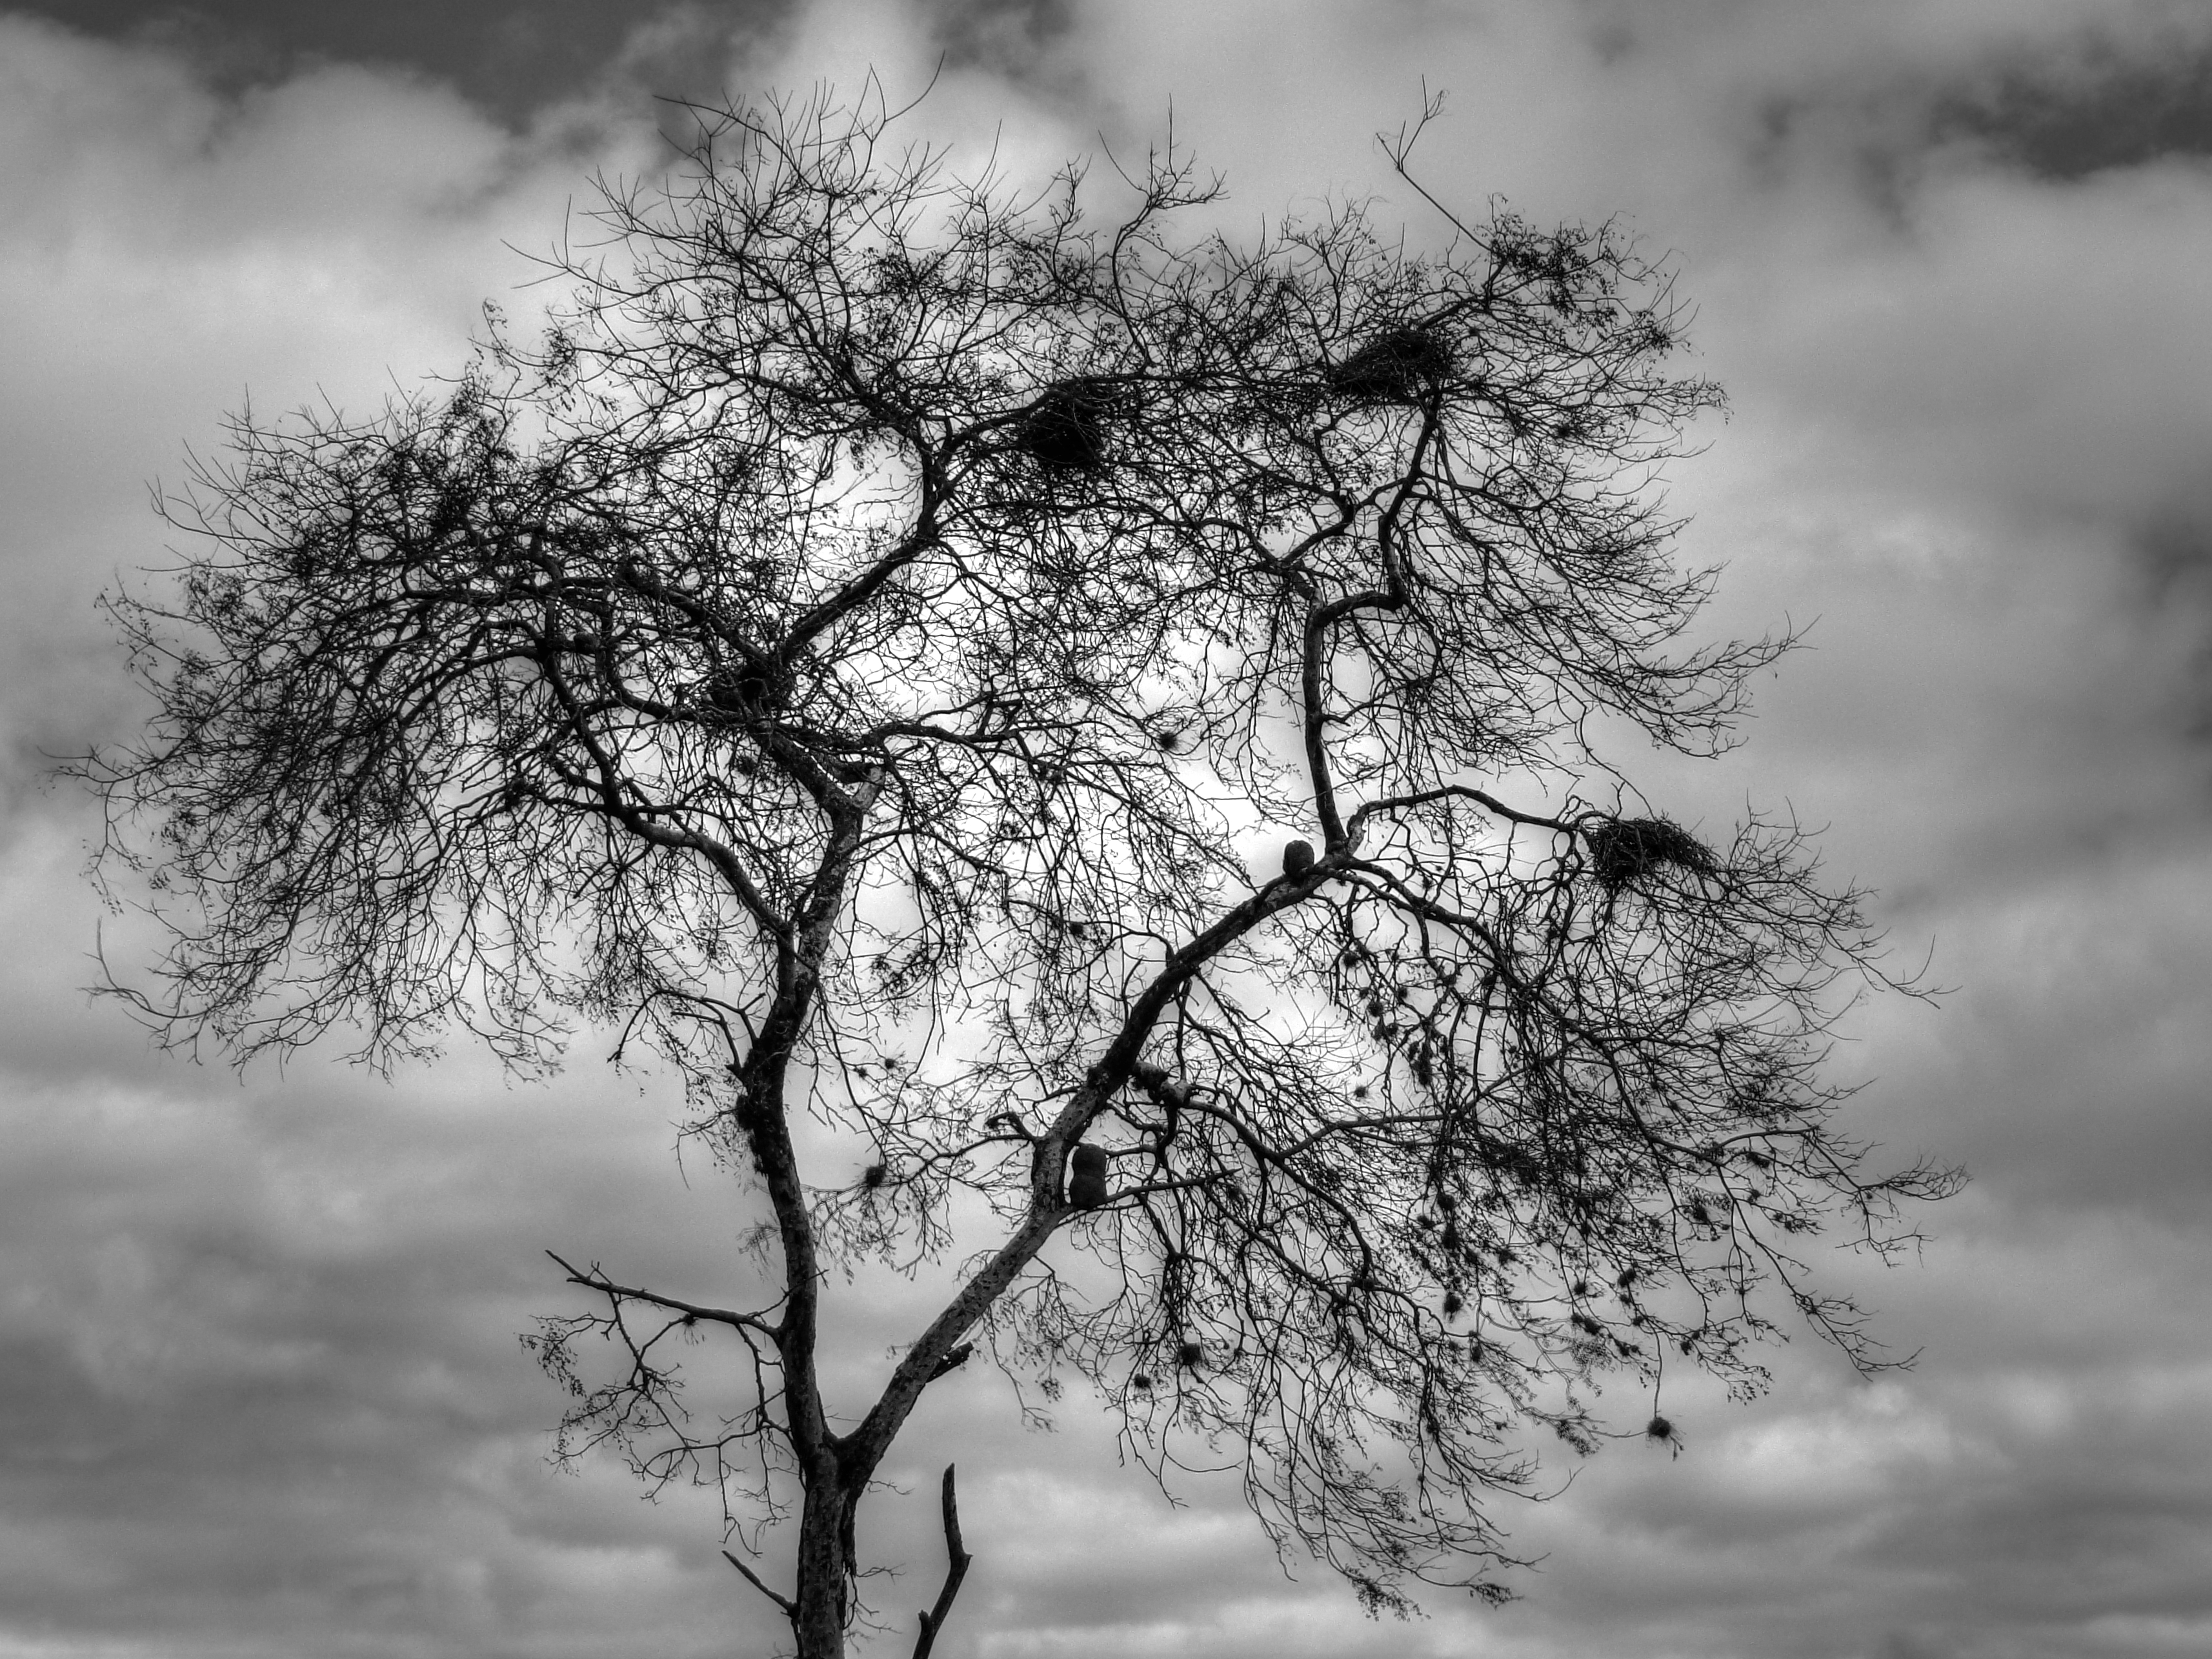
\includegraphics[width=4cm]{hdr.jpg}}
\caption{Formas euclidianas, neste caso, retas, e uma fotografia dos galhos de uma árvore. A forma natural exibe mais complexidade.}

\end{figure}

A existência desses padrões desafia a estudar estes objetos, definidos por Euclides como disformes \cite{mandelbrot1983fractal}. Segundo \citeonline[p.~1]{feder1988fractals}, diversos matemáticos propuseram alternativas que transcendem a geometria tradicional. Entretanto, tais definições não ganharam aceitação nas ciências naturais devido ao alto grau de abstração. Esta realidade mudou após a publicação dos trabalhos de Benoît B. Mandelbrot sobre a geometria fractal, conceito introduzido por ele mesmo.\par
A curva de Koch (figura \ref{koch}) e a esponja de Menger (figura \ref{menger}) são exemplos de objetos matemáticos que exibem as características observadas por Mandelbrot, que foram, previamente, classificados como "monstros matemáticos" \cite{TeseGar}.\par
A dimensão de Hausdorff-Besicovitch é um conceito matemático capaz de caracterizar a complexidade de tais objetos, associada à maneira com que os mesmos preenchem o espaço. \cite{Figueiredo2013}


\begin{figure}[!h]
\centering
\includegraphics[scale=0.5]{koch.png}
\caption{Curva de Koch. Fonte: \citeonline{TeseGar}}
\label{koch}
\end{figure}

\begin{figure}[!h]
\centering
\includegraphics[scale=0.5]{menger.png}
\caption{Esponja de Menger. Fonte: \citeonline{TeseGar}}
\label{menger}
\end{figure}
\subsection{A dimensão de Hausdorff-Besicovitch}
O conceito de dimensão topológica está associado à quantidade de informação necessária para localizar um lugar geométrico em um determinado objeto e é influenciado, como o próprio nome relata, à geometria do objeto em questão. Uma esfera, por exemplo, tem dimensão topológica 3. Já uma linha qualquer, tem dimensão topológica 1. \cite{Figueiredo2013}\par
A dimensão de Hausdorff-Besicovitch, ou simplesmente dimensão de Hausdorff, é uma extensão do conceito de dimensão e está associada à maneira com que o objeto ocupa o espaço em que está imerso, podendo ter um valor fracionário, inclusive \cite{Figueiredo2013,feder1988fractals}.\par
Segundo \citeonline[p.~12]{feder1988fractals}, a distância entre pontos no espaço é central para a definição da dimensão de Hausdorff, isto é, a maneira com que os pontos se distribuem a caracteriza.\par
O comprimento de uma linha pode ser medido a partir de segmentos de tamanho $\delta$, este é obtido a partir do número de elementos utilizados $N(\delta)$ para recobrir a linha, como mostrado na equação \ref{comprimento}.

\begin{equation}
L = N(\delta)\delta
\label{comprimento}
\end{equation}

O conceito pode ser aplicado, também, às medidas de área e de volume, a partir de pequenos quadrados e cubos, segundo as equações \ref{area} e \ref{volume}, respectivamente. 

\begin{equation}
A = N(\delta)\delta^2
\label{area}
\end{equation}

\begin{equation}
V = N(\delta)\delta^3
\label{volume}
\end{equation}

A partir das equações \ref{comprimento}, \ref{area} e \ref{volume}, pode-se definir uma forma genérica para a medida $M_{d}$, apresentada na equação \ref{md}. 

\begin{equation}
M_{d} = \lim_{\delta\rightarrow 0} N(\delta) \delta^{d}
\label{md}
\end{equation}

O expoente $d$ representa a dimensão do objeto de medida. Pode-se, então, generalizar a expressão para o número de segmentos em relação à dimensão do objeto de medida.

\begin{equation}
N(\delta) = K \delta^{-D}
\label{eqboxcount}
\end{equation}

$K$ representa uma constante de proprocionalidade. Substituindo a equação \ref{eqboxcount} na expressão genérica para a medida $M_{d}$ (equação \ref{md}).

\begin{equation}
M_{d} = \lim_{\delta\rightarrow 0} K \delta^{(d - D)}
\end{equation}

A função $M_{d}$ apresenta um ponto de transição quando $d=D$, sendo este valor a dimensão de Hausdorff do objeto, neste caso obtém-se a chamada medida de Hausdorff. O comportamento da função pode ser observado na equação \ref{transhaus}.

\begin{equation}
M_{d}(\delta) = \begin{cases} 0, & \mbox{se } d<D \\ \infty, & \mbox{se } d>D \end{cases}
\label{transhaus}
\end{equation}

A dimensão $D$ determinada com o uso da equação \ref{eqboxcount}, a partir da contagem de segmentos necessários para recobrir a figura, é chamada de dimensão de contagem de caixas ou dimensão de caixas. \cite{feder1988fractals}\par

\subsection{Box counting}

A equação \ref{eqboxcount} pode ser linearizada a partir da aplicação do logaritmo:

\begin{equation}
\log N(\delta) = \log K\delta^{-D}
\end{equation} 
\begin{equation}
\log N(\delta) = -D \log \delta + \log K
\label{bclinear}
\end{equation}

A relação \ref{bclinear} consiste em uma equação linear, onde o coeficiente desta reta corresponde à dimensão $D$ do objeto. O método de contagem de caixas, do inglês box counting, deriva desta definição e é empregado no cálculo da dimensão $D$ de um objeto genérico.\par
O cálculo de $D$ é efetuado tomando uma figura genérica e aplicando o seguinte algoritmo:

\begin{itemize}
\item Toma-se uma caixa, de dimensões iguais, que englobe a figura.
\item Divide-se a caixa em outras menores, com lados de medida iguais à metade do valor inicial.
\item O número de caixas que contém parte da figura é contado.
\item Os valores para o tamanho e o número de caixas ocupadas são registrados.
\item As caixas são, novamente, dividas ao meio e contadas. O procedimento é repetido por $n$ iterações.
\end{itemize}

A figura \ref{figurabox} ilustra o processo de contagem de caixas. Os valores para $\delta$ e $N(\delta)$ são apresentados na tabela \ref{tabbox}.

\begin{figure}[!h]
\centering
\includegraphics[scale=0.75]{boxcount.png}
\caption{Exemplo de procedimento para calculo de $D$ a partir do método de contagem de caixas para uma figura qualquer em um plano.}
\label{figurabox}
\end{figure}

\begin{table}[h]
\centering
\begin{tabular}{r|lr}
 
$\delta$ & $N(\delta)$\\
\hline                               % para uma linha horizontal
1/2 & 3\\
1/4 & 9\\
1/8 & 21
 
\end{tabular}
\caption{Valores de $\delta$ e $N(\delta)$ obtidos a partir do método box counting.}
\label{tabbox}
\end{table}

Os valores da tabela \ref{tabbox} foram ajustados para a curva da expressão \ref{bclinear} e a regressão linear apresentou um valor de $D=1,4$. O valor, se encontra, entre o apresentado para uma reta perfeita, $D=1$, e um plano perfeito, $D=2$. \par
Como fora discutido, a curva ocupa o espaço de maneira intermediária, estando entre um plano e uma reta. O gráfico destes valores pode ser encontrado na figura \ref{regbox}.
\begin{figure}[!h]
\centering
\includegraphics[scale=0.2]{graphboxcount.png}
\caption{Gráfico em escala log para os valores de $\delta$ e $N(\delta)$. A inclinação da reta apresentou um valor de $D=1,4$.}
\label{regbox}
\end{figure}

Quando realizada em um objeto fractal, a operação resulta em um valor fracionário para a dimensão de contagem de caixas. Esta é, portanto, uma característica dos fractais.\par

\subsection{Definindo um Fractal}
O termo Fractal foi cunhado por \citeonline{mandelbrot1983fractal} do adjetivo latino, fractus. O verbo frangere, em Latim, significa quebrar, criar fragmentos irregulares. Um Fractal seria, então, um objeto quebrado e irregular.\par
Um objeto Fractal é, por definição, uma forma que é feitas de partes similares ao todo e que apresenta uma dimensão de Hausdorff-Besicovitch que excede a dimensão topológica. \cite{feder1988fractals}\par 
Para um objeto que apresenta estas características, a dimensão de Hausdorff é, também, chamada dimensão fractal \cite{mandelbrot1983fractal}. Esta dimensão está associada à dinâmica que gerou a estrutura, podendo trazer informações acerca de sua complexidade \cite{Figueiredo2013}. \par
A esta característica, o objeto apresentar partes similares à figura inteira, dá-se o nome de autossimilaridade. Não é possível identificar a escala a partir de uma imagem do fractal, por exemplo, uma nuvem. A figura \ref{autosimilar} exibe a característica de autossimilaridade e invariância de escala de um fractal.

\begin{figure}[!h]
\centering
\includegraphics[scale=0.5]{autosimilar.png}
\caption{Autossimilaridade em um fractal. A figura mantém as mesmas características após sucessivas ampliações. Fonte: \citeonline{JoseGar}}
\label{autosimilar}
\end{figure}

\subsection{Auto similaridade e auto-afinidade}
Os fractais autossimilares apresentam o mesmo fator de escala em todas as direções, são, portanto, isotrópicos. O fator de escala se refere à ampliação a ser realizada para que uma estrutura similar seja obtida \cite{Figueiredo2013}. A curva de Koch e a esponja de Menger (figuras \ref{koch} e \ref{menger}, respectivamente) são exemplos de conjuntos auto-similares. \par
Entretanto, a natureza geralmente apresenta estruturas anisotrópicas, isto é, o fator de escala a ser utilizado para obtenção da mesma figura é diferente em cada direção. Essa característica é denominada autoafinidade. A figura \ref{autoafim} apresenta uma figura autoafim.\par

\begin{figure}[!h]
\centering
\includegraphics[scale=0.2]{autoafim.png}
\caption{Exemplo de estrutura auto-afim com fator de escala 4 na horizontal e 2 na vertical. Fonte: \citeonline{TeseGar}}
\label{autoafim}
\end{figure}

Algumas séries temporais de fenômenos da natureza exibem um padrão autoafim, podendo, portanto, ser caracterizadas por modelos fractais autoafins.\par

\subsection{Fractais e séries temporais: expoente de Hurst}

Segundo \citeonline{TeseGar}, apesar de não existirem "verdadeiros fractais" na natureza, alguns objetos físicos podem ser descritos com bastante precisão por fractais. Por exemplo, agregados de solo e as nuvens. \par
Uma importante aplicação da geometria fractal consiste na análise de registros temporais. Enquanto estudava problemas associados ao armazenamento de água, Hurst desenvolveu um método chamado análise R/S. O objetivo era determinar o reservatório ideal, que nunca transbordasse ou secasse \cite{feder1988fractals,Mandelbrot1968}. \par
Supondo que este reservatório recebe um volume $\xi(t)$ em um período de tempo $\tau$, o volume médio que entra será:

\begin{equation}
<\xi>_{\tau} = \frac{1}{\tau} \sum_{t=1}^{\tau} \xi(t)
\label{fluxomed}
\end{equation}

O volume de água liberado, por ano, deve ter o mesmo que o da equação \ref{fluxomed}. Tomando $x(t)$ como o volume liberado acumulado do fluxo médio de entrada:

\begin{equation}
x(t,\tau) = \sum_{u=1}^{t}\{\xi(u) - <\xi>_{\tau}\}
\label{acumulado}
\end{equation}

Hurst definiu a grandeza $R$ (do inglês, range) como a diferença entre o máximo e o mínimo valor da equação \ref{acumulado}.

\begin{equation}
R(\tau) = \max x(t,\tau) - \min x(t,\tau)
\label{range}
\end{equation}

O desvio padrão é calculado a partir de:

\begin{equation}
S = \bigg( \frac{1}{\tau} \sum_{u=1}^{t}\{\xi(u) - <\xi>_{\tau}\}^{2} \bigg)^{\frac{1}{2}}
\label{desviop}
\end{equation}

Ao estudar alguns fenômenos naturais, Hurst chegou à uma relação empírica \cite{feder1988fractals}.

\begin{equation}
\frac{R}{S} = \bigg(\frac{\tau}{2}\bigg)^{H}
\end{equation}

$H$ é chamado expoente de Hurst. Este fator fornece informações a respeito do tipo de fenômeno que gerou o registro temporal, entretanto, esta relação pode não ser encontrada em alguns fenômenos. O expoente está associado à dimensão fractal da série pela equação \ref{dimhurst}. Neste caso, $D_{A}$ indica a dimensão de auto-afinidade, que difere da dimensão de contagem de caixas uma vez que os fatores utilizados paramudança de escala não são os mesmos nas diferentes direções.

\begin{equation}
D_{A} = 2 - H
\label{dimhurst}
\end{equation}

Segundo \citeonline{mandelbrot1983fractal}, o expoente pode variar entre 0 e 1, uma vez que a dimensão fractal de uma série temporal deve variar entre 1 e 2. Um valor de H<0.5 indica um comportamento anti-persistente, H> 0.5 indica um comportamento persistente e H=0.5 está associado a um processo aleatório. \par
O expoente está, então, relacionado à correlação entre os valores medidos ao longo do tempo. Isto é, processos persistentes possuem correlação positiva entre pontos de um registro, logo, crescimentos tendem a gerar crescimentos ao passo que decrescimentos tendem a gerar decrescimentos. Já um processo anti-persistente, apresenta uma correlação negativa, logo, crescimentos tendem a anteceder decrescimentos e vice-versa \cite{mandelbrot1983fractal}.  \par
Por exemplo, a série temporal com o registro dos deslocamentos de uma partícula realizando um movimento browniano apresenta um padrão autoafim com expoente $H=0.5$, caracterizando um movimento aleatório\cite{feder1988fractals}. \par
A figura \ref{hurstvalores} exibe séries temporais de fenômenos gerados com diferentes valores de $H$.

\begin{figure}[!h]
\centering
\includegraphics[scale=0.5]{hurstvalores.png}
\caption{Exemplos de séries temporais com diferentes valores de $H$. $H=0.1$, $H=0.5$ e $H=0.9$, respectivamente. Fonte: \citeonline{JoseGar}}
\label{hurstvalores}
\end{figure}

Diversos outros métodos foram criados para estimar o expoente de Hurst de séries temporais, por exemplo: Detrended Fluctuation Analysis \cite{Peng1994} e Detrended Moving Average \cite{Alessio2002,Carbone2004}. \par
Esses métodos têm sido aplicados aos mais diversos tipos de série temporal, de registros eletrocardiográficos \cite{Peng1995} à registros financeiros \cite{Carbone2004}.

\subsection{Expoente de Hurst e sinais fisiológicos}

O expoente de Hurst foi aplicado com sucesso na análise de diversos sinais fisiológicos. De séries de intervalos entre batimentos cardíacos \cite{Peng1995} a sinais actigráficos de indivíduos saudáveis \cite{Hu2004} e com doença de Alzheimer \cite{Hu2009}. \par
A análise realizada por \citeonline{Peng1995} sugere que indivíduos cardiopatas apresentariam diferenças no expoente de Hurst e, consequentemente, nas correlações de longo alcance na série de intervalos entre batimentos cardíacos. \par
A análise de sinais de EEG, por \citeonline{Natarajan2004}, evidenciou o aumento do valor do expoente de Hurst, e, por consequência, redução da complexidade do sinal, quando eram dados estímulos sonoros aos indivíduos.\par
Foram evidenciadas, por \citeonline{Hu2004}, características de invariância de escala em séries actigráficas. Essas apresentaram um valor para o expoente de $H = 0.9 \pm 0.05$ para uma análise com janelas entre $2.5$ e $250$ minutos. \par
Uma análise similar em indivíduos idosos e com doença de Alzheimer avançada, realizada por \citeonline{Hu2009}, revelou uma redução no do expoente de Hurst. Estes pacientes apresentaram um valor de $H = 0.69 \pm 0.03$. Neste mesmo estudo, sujeitos jovens do grupo controle apresentaram $H = 0.91 \pm 0.02$, valor próximo ao reportado anteriormente \cite{Hu2004}. \par
No estudo realizado por \citeonline{Hu2009} foram monitarados, ainda, indivíduos de idade avançada e idosos sem a doença de Alzheimer. Esses apresentaram, respectivamente, valores de $H = 0.83 \pm 0.03$ e $H = 0.79 \pm 0.04$.

\section{Multifractais}

Apesar do poder da geometria fractal, algumas estruturas parecem requerer mais de um valor de $D$ para a correta caracterização, ou seja, este valor muda ao longo do conjunto. Em uma série temporal, identifica-se esta propriedade se o expoente de Hurst varia com o tempo.\par
São chamados multifractais, segundo \citeonline{Stanley1999}, objetos que requerem um número infinito de índices para a correta caracterização, tendo sido observado em diversos fenômenos físicos, por exemplo, turbulência.
Ainda segundo \citeonline{Stanley1999}, sinais fisiológicos também apresentam tais propriedades. Esses registros têm origem a partir de medidas de estruturas que possuem um complexo sistema de autorregulação.

\subsection{O fator $q$}
Segundo \citeonline{Biswas2012}, a análise de invariância de escala aplicada a séries monofractais é aplicada ao segundo momento estatístico, apenas. Pode-se expandir a análise para um momento de ordem $q$. Se as propriedades de escala se modificarem a série é multifractal. \par
Para uma série temporal qualquer, $\tau(q)$ é definido como:

\begin{equation}
<[\Delta Z(x)]^{q}>  \propto x^{\tau(q)}
\label{medida}
\end{equation}

Onde $\Delta Z(x)$ representa uma medida genérica efetuada na série temporal e $x$ o tamanho da janela analisada. \par
Se o gráfico de $\tau(q)$ versus $q$ apresenta apenas uma inclinação (linha reta) a série é monofractal \cite{Biswas2012}.

Pode-se definir, a partir de $q$, uma dimensão generalizada, ou espectro de dimensões fractais $D_{q}$ (generalização de \ref{bclinear}) como \cite{feder1988fractals,Chhabra1989}:

\begin{equation}
D_{q} = \frac{1}{q-1} \lim_{L\rightarrow0} \frac{\log\sum_{i} P_{i}^{q}(L)}{\log L}
\label{dq}
\end{equation}

Sendo $P_{i}$ a probabilidade de obter um ponto na $i$-ésima caixa. A equação \ref{dq} pode ser reescrita como:

\begin{equation}
D_{q} = \frac{1}{q-1} \tau(q)
\end{equation}

O espectro de massa ($\tau(q)$) é, então, definido como:

\begin{equation}
\tau(q) = \frac{\log\sum_{i} P_{i}^{q}(L)}{\log L}
\end{equation}

Segundo \citeonline{Chhabra1989}, o índice $q$ atua como microscópio, dando ênfase a pequenas ou grandes flutuações. Quando o $q$ é positivo, as probabilidades maiores têm seus valores aumentados e influenciam mais no cálculo do valor de $D_{q}$, em contrapartida, o valores negativos de $q$ amplificarão a influência das probabilidades menores. A figura \ref{qdq} apresenta um espectro de dimensões $D_{q}$.

\begin{figure}[!h]
\centering
\includegraphics[scale=0.3]{qDq.png}
\caption{Exemplo de espectro de dimensões generalizadas $D_{q}$. Neste caso, $q$ varia de -25 a 25.}
\label{qdq}
\end{figure}

Ainda segundo \citeonline{Biswas2012}, a dimensão generalizada, $D_{q}$, indica, para $q=0$, a chamada dimensão do suporte geométrico ou dimensão de capacidade da medida. Esta dimensão representa o padrão de distribuição na localização no espaço ou no tempo,das medidas, independente do valor absoluto dessas. Para $q=1$, $D_{q}$ está associada ao grau de heterogeneidade na distribuição da medida e é chamada dimensão de informação ou dimensão de entropia. Se $q=2$, a dimensão generalizada é conhecida como dimensão de correlação e mede a distribuição média de densidade da medida. Esta medida coincide com a dimensão de contagem de caixas do método monofractal.


\subsection{O espectro de $f(\alpha)$}

Uma outra abordagem para o estudo de multifractais consiste na análise do espectro de $f(\alpha)$ de uma determinada estrutura. 
O expoente de Lipschitz-Hölder ($\alpha$) está associado às singularidades do objeto e $f(\alpha)$ às dimensões fractais de cada uma. \cite{feder1988fractals}. Os diferentes valores de $\alpha$ definem as diferentes intensidades das singularidades de uma determinada estrutura \cite{Chhabra1989}. \par
Segundo \citeonline{Chhabra1989} e \citeonline{feder1988fractals}, o expoente de Hölder é definido a partir da equação \ref{holder}. Sendo $P_{i}$, a probabilidade de medida.

\begin{equation}
P_{i}(L) \sim L^{\alpha}
\label{holder}
\end{equation}

Uma família de medidas normalizadas pode ser construída com o parâmetro $q$. $\mu(q,L)$ representa as probabilidades em caixas de tamanho $L$ e é definido a partir de:

\begin{equation}
\mu_{i}(q,L) = \frac{[P_{i}(L)]^{q}}{\sum_{j}[P_{j}(L)]^{q}}
\label{mideq}
\end{equation}

De maneira similar à equação \ref{dq}, o parâmetro $q$ atua como um microscópio para explorar diferentes singularidades. Para $q>1$, $\mu(q)$ amplifica regiões mais singulares de $P$, enquanto para $q<1$, atribui mais peso às regiões menos singulares. Para $q=1$ a medida $\mu(1)$ reproduz os valores originais \cite{Chhabra1989}. \par
A partir do Teorema de Billingsley, pode-se relacionar a entropia de \citeonline{shannon1948}, dada pela equação \ref{shannon} à dimensão de Hausdorff, que, escrita em termos de entropia, resulta na equação \ref{hausentrpy}.

\begin{equation}
S = - \sum_{i} P_{i}log P_{i}
\label{shannon}
\end{equation}

\begin{equation}
d_{h}(M) = - \lim_{N\rightarrow\infty} \frac{1}{\log N} \sum_{i=1}^{N} P_{i}log P_{i}
\label{hausentrpy}
\end{equation}

Segundo \citeonline{Chhabra1989}, a partir das equações \ref{mideq} e \ref{hausentrpy}, pode-se definir $\alpha$ (equação \ref{alpha}) e $f(\alpha)$ (equação \ref{fdealpha}). 

\begin{equation}
\alpha(q) = \lim_{L\rightarrow 0} \frac{\sum_{i} \mu_{i} (q,L) \log {[P_{i}(L)]}}{\log L}
\label{alpha}
\end{equation}

\begin{equation}
f(\alpha(q)) = \lim_{L\rightarrow 0} \frac{\sum_{i} \mu_{i} (q,L) \log {[\mu_{i}(q,L)]}}{\log L }
\label{fdealpha}
\end{equation}

O espectro de $f(\alpha)$ consiste em um gráfico de $f(\alpha)$ versus $\alpha$ e tem formato de parábola \cite{feder1988fractals}. A figura \ref{alphaf} apresenta um exemplo de espectro de $f(\alpha)$.

\begin{figure}[!h]
\centering
\includegraphics[scale=0.3]{alphaf.png}
\caption{Exemplo de espectro de $f(\alpha)$. A curva tem o formato de uma parábola.}
\label{alphaf}
\end{figure}

$f(\alpha)$, $\tau(q)$, $\alpha$ e $q$ são variáveis termodinamicamente conjugadas e se relacionam a partir de uma transformada de Legendre a partir das expressões \ref{legendre1} e \ref{legendre2} \cite{Biswas2012,feder1988fractals, Gu2010,Chhabra1989}.

\begin{equation}
\alpha(q) = - \frac{d}{dq}\tau(q)
\label{legendre1}
\end{equation}

\begin{equation}
f(\alpha(q)) = q\alpha(q) + \tau(q)
\label{legendre2}
\end{equation}

O espectro de $f(\alpha)$ fornece informações sobre as diferentes dinâmicas que geraram a estrutura multifractal. Segundo \citeonline{Miranda2006}, a heterogeneidade de um espectro multifractal pode ser avaliada de diversas maneiras. Por exemplo, a análise da simetria e curvatura do mesmo. \par
A largura do espectro é definida como a diferença entre os valores de $\alpha$ para o maior e o menor valor de $q$. Algumas características podem ser avaliadas a partir das larguras de cada lado da parábola, definidas a partir do valor de $\alpha(q=0)$ (ou, por simplicidade, $\alpha_{0}$), sendo o lado direito ($\alpha_{0} - \alpha_{q+}$) e o lado esquerdo ($\alpha_{q-} - \alpha_{0}$), como ilustrado na figura \ref{ladosparabola} \cite{Miranda2006}.


\begin{figure}[!h]
\centering
\includegraphics[scale=0.3]{ladosparabola.png}
\caption{Análise dos lados direito ($\alpha_{0} - \alpha_{q+}$) e esquerdo ($\alpha_{q-} - \alpha_{0}$) da parábola do espectro de $f(\alpha)$ .}
\label{ladosparabola}
\end{figure}


\subsection{Multifractais e sinais fisiológicos}
O formalismo multifractal, diferente dos monofractais e expoente de Hurst, foi pouco explorado na análise de sinais fisiológicos. Sendo o trabalho realizado por \citeonline{Ivanov1999}, um exemplo de aplicação de multifractais a esses sinais. \par
Neste estudo, o espectro de $f(\alpha)$ da série temporal dos intervalos entre batimentos cardíacos de sujeitos saudáveis e cardiopatas foram analisados por \citeonline{Ivanov1999}. Os sujeitos saudáveis exibem um espectro com padrão multifractal, enquanto os indivíduos cardiopatas apresentam uma perda de multifractalidade, com a curva de $f(\alpha)$ tendendo a uma reta. \par
Um outro estudo, realizado por \citeonline{Zheng2005}, revelou um padrão multifractal para disparos de neurônios e conseguiu distinguir entre células de duas diferentes regiões cerebrais a partir das dimensões generalizadas.

\chapter{Metodologia}

Este trabalho aplica métodos não lineares e, mais especificamente, fractais e multifractais à análise de sinais actigráficos coletados de indivíduos com e sem fibromialgia. 

\section{Aqusisição dos dados}
Os dados de atividade foram coletados com o uso de dispositivos actiwatch Philips Respironics, que se assemelham a relógios de pulso e foram utilizados no braço não dominante dos indivíduos, durante todas as suas atividades, exceto o banho devido à limitação do aparelho, que não é resistente à água. \par
O dispositivo mede a movimentação do braço a partir dos acelerômetros, com os quais o mesmo é construído, e registra o valor em unidades de aceleração (u.a.). A figura \ref{actiwatch} apresenta um exemplo de série de atividade coletada de um indivíduo.\par
A coleta foi realizada no Instituto Universitario de Investigación en Ciencias de la Salud (IUNICS), Universitat de les Illes Balears, Palma de Maiorca, Espanha. O protocolo de medida foi aprovado pelo comitê de ética do Governo das Ilhas Baleares, sob número de referência, 1431/10
PI. \par
Os indivíduos, todos do sexo feminino, se dividem em dois grupos: o primeiro, de sujeitos controle, com 27 indivíduos e o segundo, com indivíduo que apresentam fibromialgia, também com 27 indivíduos. Os dados de atividade foram registrados em um período de 2 à 4 semanas, com taxa de amostragem de uma medida a cada 30 segundos. \par
Os pacientes com fibromialgia faziam uso regular de diversos medicamentos, entre eles analgésicos, ansiolíticos e antidepressivos. Entretanto, os indivíduos saudáveis não faziam uso regular de medicamentos.\par


\begin{figure}[!h]
\centering
\includegraphics[scale=0.25]{actiwatch.png}
\caption{Exemplo de série temporal de atividade de um indivíduo. Este perfil foi coletado de um indivíduo do grupo de sujeitos saudáveis.}
\label{actiwatch}
\end{figure}


\section{Análise dos sinais}

A análise dos sinais de atividade foi realizada em três etapas, consistindo, a primeira, na análise das distribuições de atividade, a segunda na obtenção dos expoentes de Hurst das séries actigráficas e a terceira na análise multifractal destes registros.\par
Inicialmente, as séries de cada indivíduos foram segmentadas em dois estados: sono, relativo ao período em que o indivíduo se encontra dormindo, e vigília, atividade que se refere ao período em que o indivíduo está acordado. Estes foram, então, empilhados em séries únicas. Cada indivíduo, então, passou a ter, além do registro original, duas séries de atividade, uma para cada estado.\par
A classificação dos intervalos de atividade do registro original, correspondentes ao diferentes estados, foi realizada pelo próprio dispositivo de coleta, a partir de um algoritmo comercial que utiliza informações do acelerômetro e de sensores de luz, também acoplados ao mesmo.\par
A figura \ref{colorstates} apresenta uma série de atividade com os segmentos relativos aos períodos de sono e vigília destacados nas cores vermelho e azul, respectivamente. Esta classificação é fornecida a partir do algoritmo do dispositivo, que foge ao escopo deste trabalho.

\begin{figure}[!h]
\centering
\includegraphics[scale=0.25]{colorstates.png}
\caption{Série temporal de atividade de um indivíduo saudável. Os estados de vigília e sono foram destacados nas cores azul e vermelha, respectivamente.}
\label{colorstates}
\end{figure}
 
A figura \ref{serieall} apresenta as séries de valores de atividade para os segmentos dos estados de vigília e sono, respectivamente, após os mesmos terem sido empilhados em um único registro.
 
\begin{figure}[!h]
\center
\subfigure[serieativo][Série resultante do empilhamento dos segmentos correspondentes ao estado de vigília.]{\includegraphics[scale=0.2]{serieativo.png}}
\quad
\subfigure[seriesono][Série resultante do empilhamento dos segmentos correspondentes ao estado de sono.]{\includegraphics[scale=0.2]{seriesono.png}}
\caption{Séries de atividade para um indivíduo com fibromialgia após a segmentação e o empilhamento do registro original.}
\label{serieall}
\end{figure} 
 
 
As distribuições acumuladas de atividade para cada indivíduo foram analisadas na tentativa de obter informações quanto à dinâmica da série. Foram estimadas, também, as distribuições de atividade em cada estado.\par
A figura \ref{distall} apresenta uma distribuição acumulada para os valores de atividade de uma série actigráfica completa de um indivíduo com fibromialgia, enquanto a figura \ref{distativosono} apresenta as distribuições acumuladas de atividade para os estados de vigília e sono de um indivíduo sem fibromialgia após a segmentação da série temporal.

\begin{figure}[!h]
\centering
\includegraphics[scale=0.3]{dist_all.png}
\caption{Distribuição de atividade para a série actigráfica de um indivíduo com fibromialgia. $P(A)$ representa a probabilidade acumulada de um valor de atividade $A$.}
\label{distall}
\end{figure}

\begin{figure}[!h]
\centering
\includegraphics[scale=0.3]{dist_ativo_sono.png}
\caption{Distribuições de atividade para os estados sono e vigília de um indivíduo saudável. $P(A)$ representa a probabilidade acumulada de um valor de atividade $A$.}
\label{distativosono}
\end{figure}

Os expoentes de Hurst foram obtidos a partir do método chamado Detrended Fluctuation Analysis (DFA), de maneira similar à utilizada por \citeonline{Hu2004}. \par
A análise multifractal da atividade foi realizada a partir de dois diferentes algoritmos. O primeiro, MFDMA\cite{Gu2010}, neste caso, uma análise multi auto-afim, já que o método se destina à caracterização de estruturas auto-afins, fora aplicado à série original. O segundo método, \citeonline{Chhabra1989}, fora aplicado às séries dos dois estados: sono e vigília.\par
A análise dos dados, a partir do método MFDMA, se limita à aplicação deste às séries temporais originais devido ao fato de o mesmo considerar a correlação na sequência temporal de eventos. Se as séries temporais são segmentadas e a estrutura original é alterada, os resultados podem ser afetados. Essa limitação não é apresentada pelo método de \citeonline{Chhabra1989}, uma vez que este analisa não as correlações temporais.

\subsection{DFA}
O método DFA foi introduzido por \citeonline{Peng1993}, este é um método eficaz para a determinação do expoente de Hurst em grandes séries de dados. \par
A série de passos do movimento (acumulada) é, primeiramente, integrada, segundo a equação \ref{integradfa}.

\begin{equation}
y(k) = \sum_{i=1}^{k} [S(i) - \bar{S}]
\label{integradfa}
\end{equation}

$S(i)$ representa o i-ésimo elemento da série e, $\bar{S}$, a média dos valores do registro. A série, é, então, dividida em janelas de tamanho $n$ e a raiz quadrática média da série integrada subtraída da tendência local, em cada janela, é calculada de acordo com a equação \ref{dfa} \cite{Peng1995}.

\begin{equation}
F(n) = \sqrt{\frac{1}{N} \sum_{k}^{N} [y(k) - y_{n}(k)]^{2}}
\label{dfa}
\end{equation}

A tendência local ($y_{n}(k)$) é calculada a partir de uma regressão linear. O número $N$ representa o número total de janelas. A equação \ref{dfa} é calculada para diversos valores para tamanhos de janela ($n$). A relação entre $F(n)$ e $n$ é caracterizada por uma lei de potência, com $H$ sendo o expoente de Hurst, em alguns fenômenos.

\begin{equation}
F(n) \sim n^{H}
\end{equation}

O método DFA foi aplicado aos dados de actigrafia na tentativa de replicar os resultados obtidos por \citeonline{Hu2004}. O tamanho das janelas utilizadas variou entre 2 e 250 minutos. Os expoentes de Hurst foram estimados a partir do algoritmo disponível no repositório PhysioNet \cite{Goldberger2000}.

\subsection{MFDMA}
O método MFDMA (Multifractal Detrended Moving Average) fora desenvolvido por \citeonline{Gu2010} e consiste em uma extensão do método DMA (Detrended Moving Average) \cite{Alessio2002} para séries multifractais. \par
A primeira etapa do algoritmo consiste em acumular a série:

\begin{equation}
y(t) = \sum_{i=1}^{t} x(i), \quad\quad t=1,2,...,N
\label{acumulada}
\end{equation}

Na segunda etapa, uma média móvel $\tilde{y}(t)$ é calculada em uma janela deslizante de tamanho $n$:

\begin{equation}
\tilde{y}(t) = \frac{1}{n} \sum_{k=0}^{n-1} y(t-k)
\label{delizante}
\end{equation} 

O procedimento de uma janela deslizante é ilustrado na figura \ref{slidingwindow}. O cálculo é efetuado com os pontos contidos em uma janela de tamanho $n$ e a mesma é deslocada por um número determinado de pontos. Esta operação é realizada por repetidas vezes até findarem-se os pontos da série.

\begin{figure}[!h]
\centering
\includegraphics[scale=0.25]{slidingwindow.png}
\caption{Exemplo de janela deslizante. O cálculo é realizado com os pontos contidos na janela 1, a mesma é, então deslocada e o cálculo é realizado novamente com os pontos contidos na janela 2.}
\label{slidingwindow}
\end{figure}

Define-se $\epsilon(i)$ como a série destendenciada da função $y(i)$, a partir da subtração de $\tilde{y}(i)$:

\begin{equation}
\epsilon(i) = y(i) - \tilde{y}(i)
\label{epsilon}
\end{equation}

A série $\epsilon(i)$ é dividida em $N_{n} = N/(n-1)$ segmentos $\epsilon_{\nu}(i)$. A raiz quadrática média será:

\begin{equation}
F_{\nu}^{2}(n) = \frac{1}{n} \sum_{i=1}^{n} \epsilon_{\nu}^{2}(i)
\label{rqm}
\end{equation}

Pode-se definir, então, o momento de ordem $q$ como:

\begin{equation}
F_{q}(n) = \bigg\{ \frac{1}{N_{n}} \sum_{\nu}^{N_{n}} F_{\nu}^{q}(n) \bigg\}^{1/q}
\label{parti}
\end{equation}

O parâmetro $q$ pode assumir o valor de qualquer número real, como na equação \ref{medida}. Quando se varia o tamanho dos segmentos $n$, obtém-se uma lei de potência para cada valor de $q$.

\begin{equation}
F_{q}(n) \sim n^{h(q)}
\end{equation}

Usando o espectro de massa ($\tau(q)$), definido, para uma série temporal, como:

\begin{equation}
\tau(q) = qh(q) - 1
\end{equation}

E aplicando a transformada de Legendre, obtem-se o espectro de $f(\alpha)$, definido como:

\begin{equation}
\alpha(q) = - \frac{d}{dq}\tau(q)
\end{equation}

\begin{equation}
f(\alpha(q)) = q\alpha(q) + \tau(q)
\end{equation}

Este algoritmo foi aplicado às series originais de atividade de todos os indivíduos para a caracterização do espectros de $f(\alpha)$ em sujeitos controle e com fibromialgia. \par
Tais espectros foram posteriormente analisados quanto à simetria e largura da parábola. Os valores obtidos para os sujeitos de cada grupo foram comparados na tentativa de estabelecer relações entre essas grandezas e as características da doença. \par
Nesta primeira análise foram utilizadas janelas de 10 minutos (20 pontos na série), como limite inferior, a cerca de 72 horas (8640 pontos na série), como limite superior. O parâmetro $q$ variou entre -5 e 5, com acréscimos de 0,1.\par 
A figura \ref{mfdmasaud} apresenta um exemplo de espectro $f(\alpha)$ para um indivíduo saudável calculado a partir do método MFDMA.

\begin{figure}[!h]
\centering
\includegraphics[scale=0.3]{spectr_saudavel_mfdma.png}
\caption{Espectro de $f(\alpha)$ obtido para um indivíduo saudável a partir do método MFDMA.}
\label{mfdmasaud}
\end{figure}

\subsection{Método de Chhabra e Jensen}

O método de \citeonline{Chhabra1989} determina os espectros multifractais diretamente a partir das expressões. \par

\begin{equation}
\alpha(q) = \lim_{L\rightarrow 0} \frac{\sum_{i} \mu_{i} (q,L) \log {[P_{i}(L)]}}{\log L}
\end{equation}

\begin{equation}
f(q) = \lim_{L\rightarrow 0} \frac{\sum_{i} \mu_{i} (q,L) \log {[\mu_{i}(q,L)]}}{\log L }
\end{equation}

Este método tem como vantagem o cálculo preciso de tais espectros, sem o uso da transformada de Legendre, sem desprezar correções logarítmicas e sem problemas com estatística ruim em pequenos e grandes valores de intensidade de singularidade \cite{Chhabra1989}. \par
O método foi aplicado às séries de atividade para o estado sono e vigília de cada um dos indivíduos, resultando em dois espectros de $f(\alpha)$ para cada sujeito, sendo um para cada estado. Estes também foram analisados quanto à sua simetria e largura. \par
Devido à grande variabilidade individual, todas as análises foram realizadas de forma pareada, isto é, as grandezas dos espectro $f(\alpha)$ do estado vigília de cada indivíduo foram comparadas com as do estado sono. \par
Este procedimento foi relizado para todos sujeitos de cada grupo, o teste pareado de Wilcoxon foi, então, aplicado para determinar quais variáveis caracterizam ou não os dois grupos. \par
Para esta análise foi utilizada uma escala inferior de 2 pontos e uma escala superior de 256 pontos. O parâmetro $q$ variou entre -25 e 25 com acréscimos de 0,1.

\begin{figure}[!h]
\centering
\includegraphics[scale=0.3]{spectr_chhabra.png}
\caption{Espectros de $f(\alpha)$ para os estados sono e vigília obtidos para um indivíduo com fibromialgia a partir do método de Chhabra-Jensen}
\label{chhabra_fibromialgia}
\end{figure}


\chapter{Resultados e Discussão}

\section{Distribuições de atividade}

As distribuições de atividade apresentaram curvas não exponenciais para ambos os grupos. As mesmas evidenciam uma enorme variabilidade entre cada um dos indivíduos. As figuras \ref{dist_h} e \ref{dist_f} apresentam as distribuições acumuladas para indivíduos saudáveis e com fibromialgia, respectivamente.

\begin{figure}[!h]
\center
\subfigure[h_semi][Distribuição em escala semi-log.]{\includegraphics[scale=0.18]{h_dist_monolog}}
\quad
\subfigure[h_log][Distribuição em escala log.]{\includegraphics[scale=0.18]{h_dist_log}}
\caption{Distribuição acumulada de atividades para indivíduos saudáveis.}
\label{dist_h}
\end{figure}

\begin{figure}[!h]
\center
\subfigure[f_semi][Distribuição em escala semi-log.]{\includegraphics[scale=0.18]{f_dist_monolog}}
\quad
\subfigure[f_log][Distribuição em escala log.]{\includegraphics[scale=0.18]{f_dist_log}}
\caption{Distribuição acumulada de atividades para indivíduos com fibromialgia.}
\label{dist_f}
\end{figure}

As distribuições apresentaram um padrão similar ao encontrado por \citeonline{Hu2004} em indivíduos saudáveis, nos dois grupos. Entretanto, a variabilidade, diferença entre curvas, é maior, principalmente, em indivíduos saudáveis.\par
Para as séries temporais dos estados ativo e sono, as curvas de distribuição de atividade apresentam as mesmas características. Estas curvas são exibidas nas figuras \ref{dist_active_h}, \ref{dist_active_f}, \ref{dist_sono_h} e \ref{dist_sono_f}.

\begin{figure}[!h]
\center
\subfigure[h_semi][Distribuição em escala semi-log.]{\includegraphics[scale=0.18]{h_dist_active_monolog}}
\quad
\subfigure[h_log][Distribuição em escala log.]{\includegraphics[scale=0.18]{h_dist_active_log}}
\caption{Distribuição acumulada de atividades para o estado ativo para indivíduos saudáveis.}
\label{dist_active_h}
\end{figure}

\begin{figure}[!h]
\center
\subfigure[f_semi][Distribuição em escala semi-log.]{\includegraphics[scale=0.18]{f_dist_active_monolog}}
\quad
\subfigure[f_log][Distribuição em escala log.]{\includegraphics[scale=0.18]{f_dist_active_log}}
\caption{Distribuição acumulada de atividades para o estado ativo para indivíduos com fibromialgia.}
\label{dist_active_f}
\end{figure}

\begin{figure}[!h]
\center
\subfigure[h_semi][Distribuição em escala semi-log.]{\includegraphics[scale=0.18]{h_dist_sleep_monolog}}
\quad
\subfigure[h_log][Distribuição em escala log.]{\includegraphics[scale=0.18]{h_dist_sleep_log}}
\caption{Distribuição acumulada de atividades para o estado sono para indivíduos saudáveis.}
\label{dist_sono_h}
\end{figure}

\begin{figure}[!h]
\center
\subfigure[f_semi][Distribuição em escala semi-log.]{\includegraphics[scale=0.18]{f_dist_sleep_monolog}}
\quad
\subfigure[f_log][Distribuição em escala log.]{\includegraphics[scale=0.18]{f_dist_sleep_log}}
\caption{Distribuição acumulada de atividades para o estado sono para indivíduos com fibromialgia.}
\label{dist_sono_f}
\end{figure}

Não foi encontrado nenhum modelo para ajustar estas curvas, todavia, as distribuições para indivíduos com fibromialgia se aproximam de curvas exponenciais, exibidas por fenômenos descorrelacionados. Estas curvas são um indicativo de que estas séries de atividade apresentem um comportamento similar ao observado por \citeonline{Peng1995}, que constatou uma redução na dimensão fractal de séries temporais de intervalos entre batimentos cardíacos de sujeitos cardiopatas. Essa redução implica em uma menor correlação de longo alcance.\par
Como já fora sugerido por \cite{Peng1993}, a perda de correlação leva a padrões de variação na série temporal compatíveis com algumas cardiopatias. Em uma análise similar, a menor correlação nas séries actigráficas de sujeitos com fibromialgia caracterizaria a síndrome e estaria associada a disfunção em mecanismos de controle motor. \par
Os valores de $R^2$ para o ajuste exponencial são exibidos na tabela \ref{tabelar2} e na figura \ref{rsquared_all}. O teste de Mann-Whitney ($\alpha=0.05$) reporta diferenças significativas ($P=0.046$), para valores de $R^2$, entre indivíduos com fibromialgia e aqueles sem a doença, variando entre 0.849 e 0.996 para sujeitos com a doença e entre 0.698 e 0.997 para sujeitos saudáveis. \par
Este resultado indica uma perda na correlaçao da atividade dos indivíduos, provavelmente provocada pela condição crônica. A privação de certos movimentos, na tentativa de evitar a dor, provocaria esta mudança nas distribuições. 

\begin{table}[h]
\centering
\begin{tabular}{|l|l|l|}
\hline
Indivíduo & Fibromialgia & Saudável \\ \hline
1         & 0.99251      & 0.99708  \\ \hline
2         & 0.99586      & 0.98310  \\ \hline
3         & 0.98828      & 0.98183  \\ \hline
4         & 0.97123      & 0.91409  \\ \hline
5         & 0.84984      & 0.94776  \\ \hline
6         & 0.99008      & 0.98179  \\ \hline
7         & 0.98014      & 0.99697  \\ \hline
8         & 0.97164      & 0.96429  \\ \hline
9         & 0.98058      & 0.69843  \\ \hline
10        & 0.99688      & 0.97479  \\ \hline
11        & 0.97578      & 0.88673  \\ \hline
12        & 0.98979      & 0.89490  \\ \hline
13        & 0.96874      & 0.71188  \\ \hline
14        & 0.99500      & 0.98409  \\ \hline
15        & 0.96425      & 0.98750  \\ \hline
16        & 0.99246      & 0.98949  \\ \hline
17        & 0.98126      & 0.98303  \\ \hline
18        & 0.98980      & 0.97011  \\ \hline
19        & 0.98908      & 0.95249  \\ \hline
20        & 0.97412      & 0.99516  \\ \hline
21        & 0.97083      & 0.98483  \\ \hline
22        & 0.98885      & 0.95980  \\ \hline
23        & 0.90596      & 0.92422  \\ \hline
24        & 0.88418      & 0.97689  \\ \hline
25        & 0.98761      & 0.94646  \\ \hline
26        & 0.99638      & 0.81849  \\ \hline
27        & 0.98429      & 0.97930  \\ \hline
\end{tabular}
\caption{Tabela com os valores do coeficiente de correlação $R^2$.}
\label{tabelar2}
\end{table}

\begin{figure}[!h]
\centering
\includegraphics[scale=0.3]{rsquared_all.png}
\caption{Valores do coeficiente de correlação $R^2$ para um ajuste exponencial das distribuições de atividade de sujeitos dos dois grupos de indivíduos.}
\label{rsquared_all}
\end{figure}

A figura \ref{rsquared_all} ilustra a maior variabilidade em sujeitos saudáveis. Observa-se facilmente que a faixa de valores de $R^2$ é muito maior nesse que em indivíduos com fibromialgia. Logo, este resultado pode sugerir uma relação entre variabilidade reduzida e a doença. \par
Estas distribuições, também, impossibilitam a caracterização das séries temporais actigráficas a partir de valores médios e desvios-padrão, como empregado por \citeonline{Kashikar-Zuck2013,Okifuji2011,Korszun2002} e \citeonline{Kashikar-zuck2010}. Estas curvas são assimétricas, e, portanto, não apresentam os primeiros e segundo momentos estatísticos.

\section{Expoentes de Hurst}
Os valores obtidos para os expoentes de Hurst são similares aos reportados por \citeonline{Hu2004} ($H = 0.9 \pm 0.05$), entretanto, não é possível distinguir entre pacientes com fibromialgia e sujeitos saudáveis por esta análise. A figura \ref{hurst_hm_fm} apresenta a variação dos valores obtidos para os dois grupos.

\begin{figure}[!h]
\centering
\includegraphics[scale=0.3]{hurst_hm_fm.png}
\caption{Valores do expoente de Hurst obtidos para sujeitos saudáveis e pacientes com fibromialgia.}
\label{hurst_hm_fm}
\end{figure}

O método não é sensível para a caracterização da fibromialgia. O resultado sugere a necessidade de outra metodologia para esta finalidade. Além disso, alguns valores de $H$, para alguns indivíduos, ultrapassaram o valor 1, isto se deve a limitações do método DFA.

\section{Espectros multifractais}

\subsection{MFDMA}

Os espectros de $f(\alpha)$ obtidos com o método MFDMA apresentaram assimetrias e uma grande variabilidade individual. As figuras \ref{h_mfdma} e \ref{f_mfdma} exibem os espectros para sujeitos saudáveis e com fibromialgia, respectivamente. \par
Para medidas nesta escala de tempo, as séries actigráficas exibem um padrão multifractal com $\alpha$ variando entre $0.8$ e $2.2$. Esta escala é diferente daquela utilizada por \citeonline{Hu2004}, que utiliza escalas superiores de horas, e analisa as flutuações ao longo de dias, avaliando variações devido a diversos fatores. \par
Assim como as distribuições de atividade, os espectros de indivíduos saudáveis apresentam maior variabilidade. A análise do espectro não permite diferenciar entre o grupo de sujeitos saudáveis e com fibromialgia devido à grande variabilidade individual. \par
Este método apresenta limitação na determinação de valores maiores de $\alpha$ devido ao uso da transformada de Legendre. O uso do método de Chhabra-Jensen é, então, uma possível evolução da metodologia por não utilizar a transformada.

\begin{figure}[!h]
\centering
\includegraphics[scale=0.3]{h_mfdma.png}
\caption{Espectros de $f(\alpha)$ para indivíduos saudáveis obtidos a partir do método MFDMA.}
\label{h_mfdma}
\end{figure}

\begin{figure}[!h]
\centering
\includegraphics[scale=0.3]{f_mfdma.png}
\caption{Espectros de $f(\alpha)$ para indivíduos com fibromialgia obtidos a partir do método MFDMA.}
\label{f_mfdma}
\end{figure}

\subsection{Método de Chhabra-Jensen}

O espectros de $f(\alpha)$ obtidos a partir deste método não apresentam os problemas que as limitações do MFDMA impõem. As curvas para indivíduos com e sem fibromialgia, nos estados de vigília e sono, são exibidas, respectivamente, nas figuras \ref{ch_fm} e \ref{ch_hm}. \par

\begin{figure}[!h]
\center
\subfigure[ch_fm_active][Espectros de $f(\alpha)$ para o estado de vigília.]{\includegraphics[scale=0.18]{ch_fm_active.png}}
\quad
\subfigure[ch_fm_sleep][Espectros de $f(\alpha)$ para o estado de sono.]{\includegraphics[scale=0.18]{ch_fm_sleep.png}}
\caption{Curvas de $f(\alpha)$ para os estados de sono e vigília de indivíduos com fibromialgia obtidos a partir do método de Chhabra-Jensen.}
\label{ch_fm}
\end{figure}

\begin{figure}[!h]
\center
\subfigure[ch_hm_active][Espectros de $f(\alpha)$ para o estado de vigília.]{\includegraphics[scale=0.18]{ch_hm_active.png}}
\quad
\subfigure[ch_hm_sleep][Espectros de $f(\alpha)$ para o estado de sono.]{\includegraphics[scale=0.18]{ch_hm_sleep.png}}
\caption{Curvas de $f(\alpha)$ para os estados de sono e vigília de sujeitos saudáveis obtidos a partir do método de Chhabra-Jensen.}
\label{ch_hm}
\end{figure}


As curvas de $f(\alpha)$, para os estados sono e vigília, são consistentes com os resultados anteriores quanto se trata de variabilidade individual, isto é, as mesmas variam muito entre os diferentes indivíduos de cada grupo.
As curvas para o estado sono são mais simétricas que as do estado de vigília. A figura \ref{ch_all} exibe as diferenças dos espectros para ambos os estados, para cada um dos grupos de indivíduos. \par

\begin{figure}[!h]
\center
\subfigure[ch_fm_all][Espectros para indivíduos com fibromialgia.]{\includegraphics[scale=0.18]{ch_fm_all.png}}
\quad
\subfigure[ch_hm_all][Espectros para indivíduos sem fibromialgia.]{\includegraphics[scale=0.18]{ch_hm_all.png}}
\caption{Curvas de $f(\alpha)$ para os estados de sono e vigília.}
\label{ch_all}
\end{figure}

Foram avaliadas as medidas dos dois lados da parábola e o valor de $\alpha_{0}$, além das dimensões generalizadas $D_{q}$ para $q=0, 1$ e $2$.
A análise dos espectros mostrou que as dinâmicas de atividade dos grupos de indivíduos são diferentes quando se comparam os estados de sono e vigília, apresentando diferenças significativas, no teste pareado de Wilcoxon, para o lado direito da parábola. A tabelas \ref{tab_lados_fm}, \ref{tab_lados_hm} e \ref{tab_dzero} apresentam as medidas de cada um dos lados das parábolas e os valores de $D_{0}$ para cada sujeito dos grupos com e sem fibromialgia, respectivamente. As figuras apresentam \ref{dir_boxplot}, \ref{esq_boxplot} e \ref{dzero_boxplot} a variação destes valores.

\begin{figure}[!h]
\centering
\includegraphics[scale=0.3]{dir_boxplot.png}
\caption{Valores da medida do lado direito da parábola ($\alpha_{q-} - \alpha_{0}$)  para sujeitos saudáveis e pacientes com fibromialgia. F indica os pacientes com fibromialgia e S os sujeitos saudáveis.}
\label{dir_boxplot}
\end{figure}

\begin{figure}[!h]
\centering
\includegraphics[scale=0.3]{esq_boxplot.png}
\caption{Valores da medida do lado esquerdo da parábola ($\alpha_{0} - \alpha_{q+}$)  para sujeitos saudáveis e pacientes com fibromialgia. F indica os pacientes com fibromialgia e S os sujeitos saudáveis.}
\label{esq_boxplot}
\end{figure}

\begin{figure}[!h]
\centering
\includegraphics[scale=0.3]{dzero_boxplot.png}
\caption{Valores da medida de $D_{0}$ para sujeitos saudáveis e pacientes com fibromialgia. F indica os pacientes com fibromialgia e S os sujeitos saudáveis.}
\label{dzero_boxplot}
\end{figure}

Os indivíduos com fibromialgia não apresentaram diferenças significativas para as medidas dos lados direitos da parábola ($\alpha_{q-} - \alpha_{0}$) entre os dois diferentes estados no teste de Wilcoxon (nível de confiança de $0.05$) ($P=0.016$). Os sujeitos saudáveis, em contrapartida, apresentaram diferenças significativas no mesmo teste. Estes valores de $\alpha$ estão associados às pequenas singularidades ($\alpha > \alpha_{0}$). \par
A dimensão de Rényi para $q=0$ ($D_{0}$) apresentou um resultado com diferenças significativas, no teste de Wilcoxon (nível de confiança de $0.05$) ($P=0.010$), apenas para indivíduos com fibromialgia. Os resultados são exibidos na tabela \ref{resumo_testes}.

\begin{table}
\centering
\begin{tabular}{ccccc}
\hline\hline
Índice & F & S\\
\hline
$\alpha_{q-} - \alpha_{0}$ & - & *\\
$D_{0}$ & * & -\\
\hline\hline
\end{tabular}
\caption{Tabela com resultados do teste pareado de Wilcoxon. F indica os indivíduos com fibromialgia, S os sujeitos saudáveis e * uma diferença significativa com nível de confiança de $0.05$)}
\label{resumo_testes}
\end{table}

O valor de $D_{0}$ representa a dimensão suporte da medida, isto é, no caso da série temporal, e indica o padrão de distribuição das regiões onde há e não há movimento, independente da quantidade deste. Tal padrão é denominado padrão de ativação do movimento. O resultado do teste de Wilcoxon indica que o grupo com fibromialgia apresenta uma dimensão de suporte diferente para os estados de sono e vigília. Logo, a ativação do movimento difere em indivíduos com a síndrome nos diferentes estados. \par
A ausência de diferença significativa entre as medidas do lado direito das parábolas para pacientes com fibromialgia nos dois estados sugere uma mesma variedade de singularidades e mesmo nível de complexidade nas duas distintas situações. \par
Estas diferenças devem ser resultado da limitação física imposta pela dor crônica apresentada por pacientes com a síndrome, relatada por \citeonline{McLoughlin2011}. As diferenças no padrão de ativação seriam explicadas pela supressão, voluntária, durante a vigília, de alguns tipos de movimento com o objetivo de atenuar a dor. As semelhanças entre os estados de sono e vigília, para as grandes singularidades, poderiam ser explicadas, também, pela supressão do movimento, os pacientes teriam, então, um padrão de movimentação no estado de vigília similar ao do sono. 


\chapter{Conclusões}
A fibromialgia é uma síndrome que submete o paciente a uma grande limitação física e, por consequência, um comprometimento de suas atividades cotidianas. Apesar de seu impacto na vida do paciente, esta é uma doença de etiologia, ainda, desconhecida. Bem como seus mecanismos e consequências a longo prazo. \par
Conhecer os mecanismos da doença é o primeiro passo na tentativa de evitá-la, mitigar seus sintomas ou até mesmo curar um sujeito portador. Entretanto, os estudos realizados, até então, se limitam ao uso de técnicas convencionais que assumem a linearidades das funções fisiológicas.\par
Diversos estudos evidenciaram características não-lineares em sinais fisiológicos. Entretanto, os estudos de atividade em pacientes com fibromialgia se limitam ao uso de medidas lineares como atividade média.\par
O uso de técnicas lineares resulta na não detecção de características do fenômeno em questão. Desta forma, o uso de técnicas não lineares, para o estudo deste tipo de dado, além de ser estatísticamente coerente, permite revelar novas características.\par
Este trabalho partiu desse pressuposto  e se propôs a analisar a atividade de indivíduos com fibromialgia a partir de técnicas originárias da teoria de sistemas complexos, e, mais especificamente, da geometria fractal.\par
Uma primeira análise dos dados já permite descartar as metodologias que aplicam análises lineares destes dados. As distribuições de atividade dos sujeitos, sejam estes saudáveis ou com fibromialgia, apresentaram não normalidade e uma grande variabilidade. Sendo esta menor em pacientes com fibromialgia.\par
As distribuições apresentaram, ainda, para pacientes com fibromialgia, um comportamento que se aproxima mais de uma curva exponencial, característica de fenômenos descorrelacionados, que os sujeitos saudáveis. Sugerindo que a fibromialgia ocasiona uma perda de correlação nos níveis de atividade dos indivíduos.\par
A análise fractal apresentou resultados similares aos de \citeonline{Hu2004}, entretanto, os expoentes de Hurst, apesar de seu poder de caracterizar fenômenos não-lineares, não são suficientes para diferir entre indivíduos com e sem fibromialgia. O problema exibe uma complexidade ainda maior e requer métodos mais avançados para a análise destes dados.\par
A análise multifractal da série temporal de atividade revela uma maior complexidade da mesma, com valores de $\alpha$ preenchendo quase todo os espectro teórico. Os espectros mantêm a variabilidade observada nas distribuições de atividade, também reduzida para indivíduos com fibromialgia.\par
Diferenças entre os dois grupos são observadas somente comparando os estados de sono e vigília de cada indivíduo de maneira pareada, com o teste de Wilcoxon. Esta forma de comparação remove a variabilidade imposta pela heterogeneidade dos indivíduos.\par
A partir desta comparação é possível observar que sujeitos saudáveis e pacientes com fibromialgia alternam características de sono e vigília de maneiras distintas. Os mecanismos de ativação do movimento no estado de vigília são os mesmos no estado de sono, apenas para sujeitos saudáveis. Os pacientes com fibromialgia apresentam padrões diferentes, com valores de dimensão de suporte maiores para o estado de sono. O que pode ser explicada pela baixa qualidade no sono dos pacientes com esse transtorno.\par
Os sujeitos saudáveis se caracterizam por mudanças na medida do lado direito do espectro multifractal, que está relacionado com o padrão de escalonamento das menores singularidades da série. Pode-se, então, concluir que para sujeitos saudáveis há uma menor densidade de pequenas singularidades, este fenômeno não é observado nas grandes singularidades.\par
Tal característica evidencia que o padrão de sono, em sujeitos saudáveis, é alterado apenas no que se refere aos movimentos suaves. É interessante notar que, para os pacientes com fibromialgia, não há diferença significativa entre estes estados, indicando que sono e vigília exibem densidades de singularidades semelhantes e próximas ao estado de sono em sujeitos saudáveis (ver Figura \ref{dir_boxplot}). O que pode ser explicado pela resistência ao movimento que a dor crônica pode provocar. \par 
A análise multifractal das séries actigráficas se mostrou capaz de distinguir entre indivíduos dos dois grupos. Entretanto, a variabilidade individual deve ser considerada. As análises devem, então, considerar esta característica dos sinais fisiológicos.\par
Diferente do que fora apresentado por \citeonline{Hu2004}, que usou escala de minutos, e apresentou uma característica fractal nas séries actigráficas, este trabalho revelou características multifractais nessas séries em escalas de tempo de até 72 horas.\par
Este trabalho avaliou características de sistemas complexos em séries temporais de actigrafia a partir de métodos multifractais. As análises revelaram uma alta complexidade de tais séries e permitiram a classificação dos grupos de indivíduos com e sem fibromialgia a partir da análise espectral, além de fornercer informações sobre a dinâmica de registros actigráficos.

\bibliographystyle{ufsc-alf}
\bibliography{fibromialgia}

\apendice
\chapter{Tabelas}

\begin{table}[h]
\centering
\begin{tabular}{|l|l|l|l|l|}
\hline
\multicolumn{5}{|c|}{Sujeitos com fibromialgia}                                       \\ \hline
           & \multicolumn{2}{c|}{Vigília} & \multicolumn{2}{c|}{Sono}    \\ \hline
Indivíduo & $\alpha_{max} - \alpha_{0}$ & $\alpha_{0} - \alpha_{min}$ & $\alpha_{max} - \alpha_{0}$ & $\alpha_{0} - \alpha_{min}$ \\ \hline
1          & 0.616226     & 0.253096      & 0.653851     & 0.549464      \\ \hline
2          & 0.636718     & 0.24801       & 0.955742     & 0.601542      \\ \hline
3          & 0.32254      & 0.137526      & 0.553996     & 0.403026      \\ \hline
4          & 0.502932     & 0.238833      & 0.696292     & 0.404399      \\ \hline
5          & 0.397553     & 0.177651      & 0.571823     & 0.494545      \\ \hline
6          & 0.371939     & 0.154855      & 0.806537     & 0.511156      \\ \hline
7          & 0.619898     & 0.177377      & 0.739995     & 0.498882      \\ \hline
8          & 1.474769     & 0.868874      & 0.69978      & 0.750393      \\ \hline
9          & 0.596144     & 0.121674      & 1.026052     & 0.457433      \\ \hline
10         & 0.843066     & 0.253576      & 0.968332     & 0.577871      \\ \hline
11         & 0.632665     & 0.219659      & 1.433072     & 0.602688      \\ \hline
12         & 1.404108     & 0.185872      & 0.505503     & 0.717279      \\ \hline
13         & 0.45716      & 0.163171      & 0.565957     & 0.520621      \\ \hline
14         & 1.703671     & 0.385842      & 0.780207     & 0.746457      \\ \hline
15         & 0.400735     & 0.20729       & 1.104128     & 0.760545      \\ \hline
16         & 0.486379     & 0.198041      & 0.292241     & 0.352878      \\ \hline
17         & 0.9478       & 0.290362      & 0.730829     & 0.97048       \\ \hline
18         & 1.993259     & 0.263183      & 0.496197     & 0.592592      \\ \hline
19         & 1.376438     & 0.161675      & 0.735182     & 0.215711      \\ \hline
20         & 0.525251     & 0.212367      & 0.761387     & 0.632001      \\ \hline
21         & 1.421908     & 0.277451      & 0.89678      & 0.627669      \\ \hline
22         & 0.636025     & 0.18369       & 0.586622     & 0.626999      \\ \hline
23         & 0.618066     & 0.191186      & 0.900618     & 0.754715      \\ \hline
24         & 1.203066     & 1.015761      & 0.644728     & 0.531057      \\ \hline
25         & 0.442981     & 0.277711      & 1.386999     & 0.41668       \\ \hline
26         & 1.698793     & 0.409835      & 0.68441      & 0.638027      \\ \hline
27         & 0.732327     & 0.248742      & 0.772862     & 0.530085      \\ \hline
\end{tabular}
\caption{Valores para as medidas dos lados esquerdo e direito da parábola, do espectro de $f(\alpha)$, obtidos a partir do método de Chhabra-Jensen, para sujeitos com fibromialgia, nos estados de sono e vigília.}
\label{tab_lados_fm}
\end{table}

\begin{table}[h]
\centering
\begin{tabular}{|l|l|l|l|l|}
\hline
\multicolumn{5}{|c|}{Sujeitos saudáveis}                                         \\ \hline
    & \multicolumn{2}{c|}{Vigília} & \multicolumn{2}{c|}{Sono}    \\ \hline
Indivíduo & $\alpha_{max} - \alpha_{0}$ & $\alpha_{0} - \alpha_{min}$ & $\alpha_{max} - \alpha_{0}$ & $\alpha_{0} - \alpha_{min}$ \\ \hline
1   & 0.299839      & 0.202694      & 0.245922     & 0.632049      \\ \hline
2   & 0.464433      & 0.117692      & 0.612982     & 0.361122      \\ \hline
3   & 2.137348      & 0.426378      & 1.508924     & 0.261619      \\ \hline
4   & 0.290857      & 0.151215      & 0.257212     & 0.635369      \\ \hline
5   & 2.010468      & 0.50353       & 0.921239     & 0.734147      \\ \hline
6   & 0.173368      & 0.120101      & 0.27662      & 0.663855      \\ \hline
7   & 2.106826      & 0.237167      & 0.933162     & 0.526636      \\ \hline
8   & 1.13093       & 0.132909      & 0.373985     & 0.69222       \\ \hline
9   & 0.190503      & 0.216308      & 0.416613     & 0.55644       \\ \hline
10  & 0.458149      & 0.194996      & 0.677698     & 0.368784      \\ \hline
11  & 0.134605      & 0.277193      & 0.208952     & 0.316266      \\ \hline
12  & 0.607561      & 0.126594      & 0.542879     & 0.53868       \\ \hline
13  & 1.887977      & 0.409044      & 1.39114      & 0.457029      \\ \hline
14  & 2.031825      & 0.245484      & 0.843821     & 0.619166      \\ \hline
15  & 0.595268      & 0.239176      & 0.682669     & 0.694957      \\ \hline
16  & 0.836184      & 0.192586      & 0.699004     & 0.496106      \\ \hline
17  & 2.48918       & 0.384306      & 1.179942     & 0.532048      \\ \hline
18  & 0.237088      & 0.195313      & 0.273635     & 0.575066      \\ \hline
19  & 1.692097      & 0.616302      & 1.093482     & 0.973394      \\ \hline
20  & 0.47524       & 0.220231      & 0.759337     & 0.421769      \\ \hline
21  & 2.523676      & 0.327856      & 0.5325       & 0.641336      \\ \hline
22  & 0.196688      & 0.159165      & 0.939084     & 0.893001      \\ \hline
23  & 1.278543      & 0.932713      & 0.898469     & 0.579757      \\ \hline
24  & 1.079373      & 1.814542      & 0.945123     & 0.65842       \\ \hline
25  & 1.010667      & 0.117817      & 0.568082     & 0.367814      \\ \hline
26  & 1.095274      & 0.193716      & 0.694314     & 0.30356       \\ \hline
27  & 1.407979      & 0.290947      & 1.135912     & 0.528626      \\ \hline
\end{tabular}
\caption{Valores para as medidas dos lados esquerdo e direito da parábola, do espectro de $f(\alpha)$, obtidos a partir do método de Chhabra-Jensen, para sujeitos sem fibromialgia, nos estados de sono e vigília.}
\label{tab_lados_hm}
\end{table}

\begin{table}[h]
\centering
\begin{tabular}{|l|l|l|l|l|}
\hline
          & \multicolumn{2}{l|}{Fibromialgia} & \multicolumn{2}{l|}{Saudáveis} \\ \hline
Indivíduo & Vigília         & Sono            & Vigília        & Sono          \\ \hline
1         & 1.00405         & 1.0061          & 1.00213        & 1.00644       \\ \hline
2         & 1.00401         & 1.0104          & 1.00161        & 1.00884       \\ \hline
3         & 1.00141         & 1.00546         & 1.00968        & 0.99752       \\ \hline
4         & 1.00333         & 1.00678         & 1.00143        & 1.00448       \\ \hline
5         & 1.0024          & 1.0058          & 1.01025        & 0.96688       \\ \hline
6         & 1.00167         & 1.00655         & 1.00059        & 1.00936       \\ \hline
7         & 0.96922         & 1.00796         & 1.00181        & 0.99596       \\ \hline
8         & 1.02289         & 1.00663         & 0.99241        & 1.01364       \\ \hline
9         & 0.96548         & 0.96165         & 1.00137        & 1.00697       \\ \hline
10        & 1.00298         & 1.00011         & 1.00306        & 1.00756       \\ \hline
11        & 1.00355         & 1.00786         & 1.0015         & 1.00211       \\ \hline
12        & 0.96358         & 1.00773         & 1.00154        & 1.0042        \\ \hline
13        & 1.00051         & 1.00835         & 1.01128        & 0.99199       \\ \hline
14        & 0.96789         & 1.00864         & 0.97304        & 0.99667       \\ \hline
15        & 1.00351         & 1.01354         & 1.00229        & 0.99851       \\ \hline
16        & 1.00332         & 1.00299         & 1.00463        & 1.0128        \\ \hline
17        & 1.00628         & 1.00111         & 0.98605        & 1.0094        \\ \hline
18        & 0.95264         & 1.00697         & 1.00136        & 1.0102        \\ \hline
19        & 1.00516         & 1.0137          & 0.98396        & 0.98089       \\ \hline
20        & 0.95422         & 0.9989          & 1.00228        & 1.00662       \\ \hline
21        & 1.00306         & 1.0108          & 0.98376        & 1.01065       \\ \hline
22        & 0.91835         & 1.01047         & 1.00078        & 1.02144       \\ \hline
23        & 1.00231         & 1.00478         & 1.05025        & 1.01171       \\ \hline
24        & 1.00171         & 1.01529         & 1.05149        & 1.00997       \\ \hline
25        & 0.99703         & 0.93029         & 0.95769        & 1.00364       \\ \hline
26        & 1.00429         & 0.99786         & 0.96967        & 1.00329       \\ \hline
27        & 0.98237         & 1.00893         & 0.97357        & 0.98616       \\ \hline
\end{tabular}
\caption{Valores de $D_{0}$ para sujeitos com e sem fibromialgia, nos estados de sono e vigília.}
\label{tab_dzero}
\end{table}

\end{document}

